% Requires in the preamble:
% \usepackage{amsmath,amssymb}
% \usepackage{tikz,pgfplots}
% \pgfplotsset{compat=1.18}

\chapter{Techniques of Integration}
\label{chap:techniques-of-integration}

Chapter \ref{chap:what-integrals-measure} showed why integrals appear everywhere.
They measure area, volume, work, mass, probability, arc length, and many other
accumulated quantities.

But setting up an integral and evaluating it are different tasks.

Substitution gave us one powerful method.  It reverses the chain rule.  But many
integrals do not come from the chain rule.  Some come from the product rule.  Some
come from trigonometric identities.  Some come from algebraic decomposition.  And
some have no elementary antiderivative at all.

So the next question is practical:

\[
\boxed{
\text{Once an application gives us an integral, how do we find its value?}
}
\]

The goal of this chapter is not to memorize tricks.  The goal is to recognize structure.
Every technique in this chapter answers the same question:

\[
\text{What derivative rule, identity, or algebraic form produced this integrand?}
\]

\section{Integration by parts}
\label{sec:integration-by-parts}

Substitution reverses the chain rule.

Integration by parts reverses the product rule.

This is the first new method because products occur naturally.  Work integrals may
contain force times distance.  Probability integrals may contain a variable times a
density.  Arc length and center of mass can also produce products.  When an integrand
looks like

\[
x e^x,\qquad x\cos x,\qquad x^2\ln x,
\]

substitution may not know what to do.  The product rule does.

\subsection{Reversing the product rule}
\label{subsec:reversing-product-rule}

The product rule says

\[
\frac{d}{dx}\bigl(u(x)v(x)\bigr)
=
u'(x)v(x)+u(x)v'(x).
\]

In differential notation, this is

\[
d(uv)=u\,dv+v\,du.
\]

This notation is useful here because it separates the two small changes: \(du\) and
\(dv\).

Rearrange the equation:

\[
u\,dv=d(uv)-v\,du.
\]

Now accumulate both sides:

\[
\int u\,dv=\int d(uv)-\int v\,du.
\]

By the Fundamental Theorem,

\[
\int d(uv)=uv.
\]

Therefore

\[
\boxed{
\int u\,dv=uv-\int v\,du.
}
\]

This is the formula for integration by parts.

\begin{quote}
\textbf{Integration by parts.}
If \(u=u(x)\) and \(v=v(x)\) are differentiable functions, then

\[
\boxed{
\int u\,dv=uv-\int v\,du.
}
\]

Equivalently, if \(dv=v'(x)\,dx\) and \(du=u'(x)\,dx\), then

\[
\boxed{
\int u(x)v'(x)\,dx
=
u(x)v(x)-\int v(x)u'(x)\,dx.
}
\]
\end{quote}

The formula does not make an integral disappear for free.  It trades one integral for
another.  It helps only when the new integral is simpler than the old one.

\paragraph{Seed example.}
Find

\[
\int x e^x\,dx.
\]

The integrand is a product.  The factor \(e^x\) is easy to integrate, and the factor
\(x\) becomes simpler when differentiated.

Choose

\[
u=x,
\qquad
dv=e^x\,dx.
\]

Then

\[
du=dx,
\qquad
v=e^x.
\]

Integration by parts gives

\[
\int x e^x\,dx
=
x e^x-\int e^x\,dx.
\]

So

\[
\boxed{
\int x e^x\,dx
=
x e^x-e^x+C.
}
\]

It is worth checking:

\[
\frac{d}{dx}\bigl(xe^x-e^x\bigr)
=
(e^x+xe^x)-e^x
=
xe^x.
\]

The derivative returns the original integrand.

\subsection{Choosing \texorpdfstring{\(u\)}{u} and \texorpdfstring{\(dv\)}{dv}}
\label{subsec:choosing-u-dv}

The formula

\[
\int u\,dv=uv-\int v\,du
\]

requires a choice.  We must decide which part of the integrand to call \(u\), and
which part to call \(dv\).

The choice is not cosmetic.  A good choice makes the remaining integral simpler.
A poor choice makes it harder.

In the example

\[
\int x e^x\,dx,
\]

we chose

\[
u=x,
\qquad
dv=e^x\,dx.
\]

That made

\[
du=dx,
\]

so the power of \(x\) disappeared.

If we had chosen instead

\[
u=e^x,
\qquad
dv=x\,dx,
\]

then

\[
du=e^x\,dx,
\qquad
v=\frac{x^2}{2}.
\]

The formula would give

\[
\int x e^x\,dx
=
\frac{x^2}{2}e^x-\int \frac{x^2}{2}e^x\,dx.
\]

The new integral is harder than the original one.  That choice moves us backward.

\begin{quote}
\textbf{Choosing \(u\) and \(dv\).}
Ask two questions.

\begin{center}
\begin{tabular}{c|l}
\textbf{Question} & \textbf{Reason} \\ \hline
Will \(u\) become simpler when differentiated? & We must replace \(u\) by \(du\). \\[3pt]
Can \(dv\) be integrated easily? & We must find \(v\).
\end{tabular}
\end{center}

A good choice usually makes \(du\) simpler than \(u\), while keeping \(v\) manageable.
\end{quote}

\paragraph{Example: no visible product.}
Find

\[
\int \ln x\,dx,
\qquad x>0.
\]

There is no visible product, but we can write

\[
\ln x=(\ln x)\cdot 1.
\]

Choose

\[
u=\ln x,
\qquad
dv=dx.
\]

Then

\[
du=\frac1x\,dx,
\qquad
v=x.
\]

Integration by parts gives

\[
\int \ln x\,dx
=
x\ln x-\int x\cdot \frac1x\,dx.
\]

Thus

\[
\int \ln x\,dx
=
x\ln x-\int 1\,dx,
\]

so

\[
\boxed{
\int \ln x\,dx=x\ln x-x+C.
}
\]

This example is a useful reminder.  Integration by parts can apply even when the
integrand does not look like a product.  The hidden factor may be \(1\,dx\).

\paragraph{Example: a trigonometric product.}
Find

\[
\int x\cos x\,dx.
\]

Choose

\[
u=x,
\qquad
dv=\cos x\,dx.
\]

Then

\[
du=dx,
\qquad
v=\sin x.
\]

So

\[
\int x\cos x\,dx
=
x\sin x-\int \sin x\,dx.
\]

Since

\[
\int \sin x\,dx=-\cos x,
\]

we get

\[
\boxed{
\int x\cos x\,dx=x\sin x+\cos x+C.
}
\]

The sign comes from the antiderivative of \(\sin x\).  A quick derivative check confirms
the result:

\[
\frac{d}{dx}(x\sin x+\cos x)
=
\sin x+x\cos x-\sin x
=
x\cos x.
\]

\subsection{Repeated integration by parts}
\label{subsec:repeated-integration-by-parts}

Sometimes one use of integration by parts is not enough.  A power may need to be
reduced one degree at a time.

\paragraph{Example.}
Find

\[
\int x^2 e^x\,dx.
\]

Choose

\[
u=x^2,
\qquad
dv=e^x\,dx.
\]

Then

\[
du=2x\,dx,
\qquad
v=e^x.
\]

So

\[
\int x^2 e^x\,dx
=
x^2e^x-\int 2x e^x\,dx.
\]

The remaining integral still needs integration by parts.  From the seed example,

\[
\int x e^x\,dx=xe^x-e^x+C.
\]

Therefore

\[
\int 2x e^x\,dx
=
2xe^x-2e^x.
\]

Substitute back:

\[
\int x^2 e^x\,dx
=
x^2e^x-(2xe^x-2e^x)+C.
\]

Thus

\[
\boxed{
\int x^2 e^x\,dx
=
e^x(x^2-2x+2)+C.
}
\]

The pattern is clear.  Each integration by parts differentiates the polynomial factor.
Eventually the polynomial becomes constant.

\paragraph{A cyclic example.}
Some integrals do not become simpler at each step.  Instead, the original integral
returns.

Let

\[
I=\int e^x\cos x\,dx.
\]

Choose

\[
u=\cos x,
\qquad
dv=e^x\,dx.
\]

Then

\[
du=-\sin x\,dx,
\qquad
v=e^x.
\]

So

\[
I=e^x\cos x+\int e^x\sin x\,dx.
\]

Now integrate the remaining integral.  Let

\[
J=\int e^x\sin x\,dx.
\]

Choose

\[
u=\sin x,
\qquad
dv=e^x\,dx.
\]

Then

\[
du=\cos x\,dx,
\qquad
v=e^x.
\]

Thus

\[
J=e^x\sin x-\int e^x\cos x\,dx.
\]

But the last integral is \(I\).  Therefore

\[
J=e^x\sin x-I.
\]

Substitute this into the equation for \(I\):

\[
I=e^x\cos x+J
=
e^x\cos x+e^x\sin x-I.
\]

So

\[
2I=e^x(\sin x+\cos x).
\]

Hence

\[
\boxed{
\int e^x\cos x\,dx
=
\frac12 e^x(\sin x+\cos x)+C.
}
\]

When the original integral returns, do not panic.  Treat it as an unknown and solve for
it.

\subsection{Definite integrals and boundary terms}
\label{subsec:definite-integrals-boundary-terms}

For definite integrals, integration by parts has the same idea, but the product term is
evaluated at the endpoints.

\begin{quote}
\textbf{Integration by parts for definite integrals.}
If \(u\) and \(v\) are differentiable on \([a,b]\), then

\[
\boxed{
\int_a^b u\,dv
=
\bigl[uv\bigr]_a^b-\int_a^b v\,du.
}
\]

Here

\[
\bigl[uv\bigr]_a^b=u(b)v(b)-u(a)v(a).
\]
\end{quote}

The term \(\bigl[uv\bigr]_a^b\) is called a \emph{boundary term}.  It comes from the
Fundamental Theorem:

\[
\int_a^b d(uv)=u(b)v(b)-u(a)v(a).
\]

In an indefinite integral, this term appears as \(uv\).  In a definite integral, it becomes
an endpoint contribution.

\paragraph{Example.}
Evaluate

\[
\int_0^1 x e^x\,dx.
\]

Use

\[
u=x,
\qquad
dv=e^x\,dx.
\]

Then

\[
du=dx,
\qquad
v=e^x.
\]

So

\[
\int_0^1 x e^x\,dx
=
\bigl[x e^x\bigr]_0^1-\int_0^1 e^x\,dx.
\]

Compute the boundary term:

\[
\bigl[x e^x\bigr]_0^1=e-0=e.
\]

Also,

\[
\int_0^1 e^x\,dx=e-1.
\]

Therefore

\[
\int_0^1 x e^x\,dx
=
e-(e-1)=\boxed{1}.
\]

No \(+C\) appears in a definite integral.  The endpoint evaluation produces a number.

\paragraph{Example: the boundary term carries the main value.}
Evaluate

\[
\int_0^\pi x\sin x\,dx.
\]

Choose

\[
u=x,
\qquad
dv=\sin x\,dx.
\]

Then

\[
du=dx,
\qquad
v=-\cos x.
\]

Therefore

\[
\int_0^\pi x\sin x\,dx
=
\bigl[-x\cos x\bigr]_0^\pi-\int_0^\pi (-\cos x)\,dx.
\]

The boundary term is

\[
\bigl[-x\cos x\bigr]_0^\pi
=
-\pi\cos\pi-0
=
\pi.
\]

The remaining integral is

\[
\int_0^\pi \cos x\,dx
=
\sin x\Big|_0^\pi
=
0.
\]

So

\[
\boxed{
\int_0^\pi x\sin x\,dx=\pi.
}
\]

The value comes entirely from the boundary term.

\begin{quote}
\textbf{A common mistake.}
Do not write

\[
\int_a^b u\,dv=uv-\int_a^b v\,du.
\]

The expression \(uv\) is a function, not a number.  For a definite integral it must be
evaluated at the endpoints:

\[
\int_a^b u\,dv=\bigl[uv\bigr]_a^b-\int_a^b v\,du.
\]
\end{quote}

Integration by parts is one way of recognizing the hidden derivative rule behind an
integrand.  Products of algebraic and exponential or logarithmic functions often need it.

But another large family of integrals comes from identities rather than product rules.
Trigonometric functions bring their own algebra.

\section{Trigonometric integrals}
\label{sec:trigonometric-integrals}

Trigonometric functions have two kinds of structure at once.

First, their derivatives cycle:

\[
\frac{d}{dx}\sin x=\cos x,
\qquad
\frac{d}{dx}\cos x=-\sin x.
\]

Second, their values are tied together by identities:

\[
\sin^2 x+\cos^2 x=1,
\]

\[
1+\tan^2 x=\sec^2 x.
\]

Trigonometric integrals use both facts.  We try to save a factor that becomes a
differential, and then use an identity to rewrite everything else.

\subsection{Powers of sine and cosine}
\label{subsec:powers-sine-cosine}

The standard form is

\[
\int \sin^m x\cos^n x\,dx,
\]

where \(m\) and \(n\) are nonnegative integers.

The key is to look for an odd power.  An odd power lets us save one factor for the
differential.

\subsubsection*{An odd power of cosine}

Consider

\[
\int \sin^4 x\cos^3 x\,dx.
\]

The power of cosine is odd.  Save one factor of \(\cos x\,dx\):

\[
\cos^3 x\,dx=\cos^2 x\cos x\,dx.
\]

Use

\[
\cos^2 x=1-\sin^2 x.
\]

Then

\[
\int \sin^4 x\cos^3 x\,dx
=
\int \sin^4 x(1-\sin^2 x)\cos x\,dx.
\]

Now substitute

\[
u=\sin x,
\qquad
du=\cos x\,dx.
\]

The integral becomes

\[
\int u^4(1-u^2)\,du.
\]

So

\[
\int u^4(1-u^2)\,du
=
\int (u^4-u^6)\,du
=
\frac{u^5}{5}-\frac{u^7}{7}+C.
\]

Return to \(x\):

\[
\boxed{
\int \sin^4 x\cos^3 x\,dx
=
\frac{\sin^5 x}{5}-\frac{\sin^7 x}{7}+C.
}
\]

The method worked because one \(\cos x\,dx\) became \(du\), and all remaining
cosines were converted into sines.

\subsubsection*{An odd power of sine}

Now consider

\[
\int \sin^3 x\cos^2 x\,dx.
\]

The power of sine is odd.  Save one factor of \(\sin x\,dx\):

\[
\sin^3 x\,dx=\sin^2 x\sin x\,dx.
\]

Use

\[
\sin^2 x=1-\cos^2 x.
\]

Then

\[
\int \sin^3 x\cos^2 x\,dx
=
\int (1-\cos^2 x)\cos^2 x\sin x\,dx.
\]

Choose

\[
u=\cos x,
\qquad
du=-\sin x\,dx.
\]

Since \(\sin x\,dx=-du\), the integral becomes

\[
-\int (1-u^2)u^2\,du.
\]

So

\[
-\int (u^2-u^4)\,du
=
-\frac{u^3}{3}+\frac{u^5}{5}+C.
\]

Return to \(x\):

\[
\boxed{
\int \sin^3 x\cos^2 x\,dx
=
-\frac{\cos^3 x}{3}+\frac{\cos^5 x}{5}+C.
}
\]

The negative sign comes from

\[
d(\cos x)=-\sin x\,dx.
\]

\subsubsection*{Both powers even}

If both powers are even, no single sine or cosine factor is available for substitution.
Then half-angle identities are the usual tool:

\[
\sin^2 x=\frac{1-\cos 2x}{2},
\qquad
\cos^2 x=\frac{1+\cos 2x}{2}.
\]

\paragraph{Example.}
Find

\[
\int \sin^2 x\cos^2 x\,dx.
\]

First use

\[
\sin x\cos x=\frac12\sin 2x.
\]

Then

\[
\sin^2 x\cos^2 x
=
\frac14\sin^2 2x.
\]

Now use

\[
\sin^2 2x=\frac{1-\cos 4x}{2}.
\]

Therefore

\[
\sin^2 x\cos^2 x
=
\frac18(1-\cos 4x).
\]

So

\[
\int \sin^2 x\cos^2 x\,dx
=
\frac18\int (1-\cos 4x)\,dx.
\]

Thus

\[
\boxed{
\int \sin^2 x\cos^2 x\,dx
=
\frac{x}{8}-\frac{\sin 4x}{32}+C.
}
\]

\begin{quote}
\textbf{Powers of sine and cosine.}

\begin{center}
\begin{tabular}{c|l}
\textbf{Situation} & \textbf{First move} \\ \hline
\(\cos x\) has an odd power & Save one \(\cos x\,dx\), convert remaining cosines using \(\cos^2x=1-\sin^2x\). \\[4pt]
\(\sin x\) has an odd power & Save one \(\sin x\,dx\), convert remaining sines using \(\sin^2x=1-\cos^2x\). \\[4pt]
Both powers are even & Use half-angle identities.
\end{tabular}
\end{center}
\end{quote}

The point is not the table.  The point is the saved differential.  We save the piece that
matches the derivative of the other trigonometric function.

\subsection{Powers of tangent and secant}
\label{subsec:powers-tangent-secant}

The next common family is

\[
\int \tan^m x\sec^n x\,dx.
\]

The useful derivative pairs are

\[
\frac{d}{dx}\tan x=\sec^2 x,
\]

and

\[
\frac{d}{dx}\sec x=\sec x\tan x.
\]

The useful identity is

\[
\sec^2 x=1+\tan^2 x,
\]

or equivalently

\[
\tan^2 x=\sec^2 x-1.
\]

Again, we try to save a differential.

\subsubsection*{An even power of secant}

If the power of \(\sec x\) is even, save one factor of \(\sec^2 x\,dx\).  Then convert the
remaining powers of secant into tangent.

\paragraph{Example.}
Find

\[
\int \tan^3 x\sec^4 x\,dx.
\]

Write

\[
\sec^4 x=\sec^2 x\sec^2 x.
\]

Save one \(\sec^2 x\,dx\):

\[
\int \tan^3 x\sec^4 x\,dx
=
\int \tan^3 x\sec^2 x\,\sec^2 x\,dx.
\]

Convert the remaining \(\sec^2 x\) into \(1+\tan^2 x\):

\[
\int \tan^3 x(1+\tan^2 x)\sec^2 x\,dx.
\]

Now let

\[
u=\tan x,
\qquad
du=\sec^2 x\,dx.
\]

Then the integral becomes

\[
\int u^3(1+u^2)\,du
=
\int (u^3+u^5)\,du.
\]

Therefore

\[
\boxed{
\int \tan^3 x\sec^4 x\,dx
=
\frac{\tan^4 x}{4}+\frac{\tan^6 x}{6}+C.
}
\]

\subsubsection*{An odd power of tangent}

If the power of \(\tan x\) is odd and at least one factor of \(\sec x\) is present, save

\[
\sec x\tan x\,dx.
\]

Then use

\[
\tan^2 x=\sec^2 x-1
\]

to rewrite the remaining tangent powers in terms of secant.

\paragraph{Example.}
Find

\[
\int \sec^5 x\tan^3 x\,dx.
\]

Save one \(\sec x\tan x\,dx\):

\[
\int \sec^5 x\tan^3 x\,dx
=
\int \sec^4 x\tan^2 x(\sec x\tan x)\,dx.
\]

Use

\[
\tan^2 x=\sec^2 x-1.
\]

Then

\[
\int \sec^4 x(\sec^2 x-1)(\sec x\tan x)\,dx.
\]

Let

\[
u=\sec x,
\qquad
du=\sec x\tan x\,dx.
\]

The integral becomes

\[
\int u^4(u^2-1)\,du
=
\int (u^6-u^4)\,du.
\]

So

\[
\boxed{
\int \sec^5 x\tan^3 x\,dx
=
\frac{\sec^7 x}{7}-\frac{\sec^5 x}{5}+C.
}
\]

\subsubsection*{A small special case}

Sometimes the identity alone is enough.

\[
\int \tan^2 x\,dx
=
\int(\sec^2 x-1)\,dx.
\]

Therefore

\[
\boxed{
\int \tan^2 x\,dx=\tan x-x+C.
}
\]

This is a good example of strategy over memorization.  We do not need a new formula
for \(\int \tan^2 x\,dx\).  We use the identity that connects \(\tan x\) to a derivative
we already know.

\subsubsection*{When integration by parts returns}

Some tangent-secant integrals need integration by parts.  A famous example is

\[
\int \sec^3 x\,dx.
\]

Let

\[
I=\int \sec^3 x\,dx
=
\int \sec x\sec^2 x\,dx.
\]

Choose

\[
u=\sec x,
\qquad
dv=\sec^2 x\,dx.
\]

Then

\[
du=\sec x\tan x\,dx,
\qquad
v=\tan x.
\]

Integration by parts gives

\[
I=\sec x\tan x-\int \sec x\tan^2 x\,dx.
\]

Use

\[
\tan^2 x=\sec^2 x-1.
\]

Then

\[
I
=
\sec x\tan x-\int \sec x(\sec^2 x-1)\,dx.
\]

So

\[
I
=
\sec x\tan x-\int \sec^3 x\,dx+\int \sec x\,dx.
\]

The original integral returns:

\[
I=\sec x\tan x-I+\int \sec x\,dx.
\]

Thus

\[
2I=\sec x\tan x+\int \sec x\,dx.
\]

We still need

\[
\int \sec x\,dx.
\]

Multiply by a clever form of \(1\):

\[
\int \sec x\,dx
=
\int \sec x\cdot\frac{\sec x+\tan x}{\sec x+\tan x}\,dx.
\]

The numerator becomes

\[
\sec^2 x+\sec x\tan x,
\]

which is the derivative of

\[
\sec x+\tan x.
\]

Therefore

\[
\int \sec x\,dx
=
\ln|\sec x+\tan x|+C.
\]

So

\[
2I=\sec x\tan x+\ln|\sec x+\tan x|.
\]

Hence

\[
\boxed{
\int \sec^3 x\,dx
=
\frac12\sec x\tan x+\frac12\ln|\sec x+\tan x|+C.
}
\]

This example combines the methods: identity, integration by parts, and substitution.

\subsection{Product-to-sum identities}
\label{subsec:product-to-sum-identities}

Products such as

\[
\sin(5x)\cos(2x)
\]

do not fit the power patterns above.  The angles are different.  In this case,
product-to-sum identities turn products into sums, and sums are easier to integrate.

The main identities are

\[
\sin A\cos B
=
\frac12\bigl(\sin(A+B)+\sin(A-B)\bigr),
\]

\[
\cos A\cos B
=
\frac12\bigl(\cos(A-B)+\cos(A+B)\bigr),
\]

and

\[
\sin A\sin B
=
\frac12\bigl(\cos(A-B)-\cos(A+B)\bigr).
\]

\paragraph{Example.}
Find

\[
\int \sin(5x)\cos(2x)\,dx.
\]

Use

\[
\sin A\cos B
=
\frac12\bigl(\sin(A+B)+\sin(A-B)\bigr)
\]

with

\[
A=5x,
\qquad
B=2x.
\]

Then

\[
\sin(5x)\cos(2x)
=
\frac12\bigl(\sin(7x)+\sin(3x)\bigr).
\]

So

\[
\int \sin(5x)\cos(2x)\,dx
=
\frac12\int \bigl(\sin(7x)+\sin(3x)\bigr)\,dx.
\]

Integrate term by term:

\[
\boxed{
\int \sin(5x)\cos(2x)\,dx
=
-\frac{\cos(7x)}{14}-\frac{\cos(3x)}{6}+C.
}
\]

The identity did the hard work.  Once the product became a sum, the integral was
routine.

\subsection{Strategy over memorization}
\label{subsec:trig-integral-strategy}

Trigonometric integrals can look like a long list of cases.  But the cases are guided by
a few questions.

\begin{quote}
\textbf{Questions to ask.}

\begin{center}
\begin{tabular}{p{0.34\textwidth}|p{0.56\textwidth}}
\textbf{What do you see?} & \textbf{What should you try?} \\ \hline
A power of \(\sin x\) and a power of \(\cos x\) & Look for an odd power.  Save one factor for \(du\), and convert the rest using \(\sin^2x+\cos^2x=1\). \\[6pt]
Only even powers of \(\sin x\) and \(\cos x\) & Use half-angle identities. \\[6pt]
A power of \(\tan x\) and a power of \(\sec x\) & Look for \(\sec^2x\,dx\) or \(\sec x\tan x\,dx\). \\[6pt]
Different angles, such as \(\sin(5x)\cos(2x)\) & Use product-to-sum identities. \\[6pt]
A case that returns the original integral & Name the integral \(I\), continue, and solve for \(I\).
\end{tabular}
\end{center}
\end{quote}

The deeper habit is this:

\[
\boxed{
\text{Save a differential, then use identities to rewrite everything else.}
}
\]

That habit is the same one we used in substitution.  The difference is that
trigonometric identities give us the algebra needed to make substitution possible.

\paragraph{A final mixed example.}
Find

\[
\int \sin^5 x\cos^2 x\,dx.
\]

The power of sine is odd.  Save one \(\sin x\,dx\), and convert the remaining powers
of sine into cosines:

\[
\sin^5 x=\sin^4 x\sin x=(\sin^2 x)^2\sin x.
\]

Since

\[
\sin^2 x=1-\cos^2 x,
\]

we get

\[
\int \sin^5 x\cos^2 x\,dx
=
\int (1-\cos^2 x)^2\cos^2 x\sin x\,dx.
\]

Let

\[
u=\cos x,
\qquad
du=-\sin x\,dx.
\]

Then

\[
\int (1-\cos^2 x)^2\cos^2 x\sin x\,dx
=
-\int (1-u^2)^2u^2\,du.
\]

Expand:

\[
(1-u^2)^2u^2=(1-2u^2+u^4)u^2=u^2-2u^4+u^6.
\]

So

\[
-\int (u^2-2u^4+u^6)\,du
=
-\frac{u^3}{3}+\frac{2u^5}{5}-\frac{u^7}{7}+C.
\]

Return to \(x\):

\[
\boxed{
\int \sin^5 x\cos^2 x\,dx
=
-\frac{\cos^3 x}{3}
+\frac{2\cos^5 x}{5}
-\frac{\cos^7 x}{7}
+C.
}
\]

The computation looks long, but the idea is short.  Save \(\sin x\,dx\), rewrite the
rest in terms of \(\cos x\), and substitute.

Trigonometric identities help with powers of trigonometric functions.  In the next
section, they will do something more surprising: they will remove square roots such as

\[
\sqrt{9-x^2},
\qquad
\sqrt{x^2+4},
\qquad
\sqrt{x^2-1}.
\]

That happens because the identities

\[
1-\sin^2\theta=\cos^2\theta,
\qquad
1+\tan^2\theta=\sec^2\theta,
\qquad
\sec^2\theta-1=\tan^2\theta
\]

are also identities about right triangles.  This leads to trigonometric substitution.
\section{Trigonometric substitution}
\label{sec:trigonometric-substitution}

Trigonometric integrals used identities after trigonometric functions were already
present.  Trigonometric substitution uses those identities earlier.  It creates
trigonometric functions on purpose.

The reason is square roots.

Integrals such as

\[
\int \sqrt{9-x^2}\,dx,
\qquad
\int \frac{dx}{\sqrt{x^2+4}},
\qquad
\int \sqrt{x^2-1}\,dx
\]

do not look trigonometric.  But the expressions under the square roots resemble the
three Pythagorean identities:

\[
1-\sin^2\theta=\cos^2\theta,
\]

\[
1+\tan^2\theta=\sec^2\theta,
\]

\[
\sec^2\theta-1=\tan^2\theta.
\]

A trigonometric substitution chooses \(x\) so that the square root becomes a simpler
trigonometric expression.  The square root does not vanish by magic.  It vanishes
because a right triangle or a circle was hidden inside it.

\subsection{Square roots from circles and triangles}
\label{subsec:square-roots-circles-triangles}

Start with

\[
\sqrt{9-x^2}.
\]

This expression comes from the circle

\[
x^2+y^2=9.
\]

Solving for the upper half gives

\[
y=\sqrt{9-x^2}.
\]

A point on the circle of radius \(3\) can be described by

\[
x=3\sin\theta.
\]

Then

\[
9-x^2
=
9-9\sin^2\theta
=
9(1-\sin^2\theta)
=
9\cos^2\theta.
\]

So

\[
\sqrt{9-x^2}
=
3|\cos\theta|.
\]

If we choose

\[
-\frac{\pi}{2}\le \theta\le \frac{\pi}{2},
\]

then \(\cos\theta\ge0\), and therefore

\[
\sqrt{9-x^2}=3\cos\theta.
\]

That is the whole idea.  We choose the range of \(\theta\) so that the square root is
nonnegative without needing an absolute value.

\paragraph{Seed example.}
Find

\[
\int \sqrt{9-x^2}\,dx.
\]

Use

\[
x=3\sin\theta,
\qquad
-\frac{\pi}{2}\le \theta\le \frac{\pi}{2}.
\]

Then

\[
dx=3\cos\theta\,d\theta,
\]

and

\[
\sqrt{9-x^2}=3\cos\theta.
\]

The integral becomes

\[
\int \sqrt{9-x^2}\,dx
=
\int (3\cos\theta)(3\cos\theta)\,d\theta.
\]

So

\[
\int \sqrt{9-x^2}\,dx
=
9\int \cos^2\theta\,d\theta.
\]

Use the half-angle identity

\[
\cos^2\theta=\frac{1+\cos 2\theta}{2}.
\]

Then

\[
9\int \cos^2\theta\,d\theta
=
\frac92\int(1+\cos 2\theta)\,d\theta.
\]

Thus

\[
9\int \cos^2\theta\,d\theta
=
\frac92\theta+\frac94\sin2\theta+C.
\]

Now return to \(x\).  Since

\[
x=3\sin\theta,
\]

we have

\[
\theta=\arcsin\left(\frac{x}{3}\right).
\]

Also,

\[
\sin2\theta=2\sin\theta\cos\theta.
\]

From the substitution,

\[
\sin\theta=\frac{x}{3}
\]

and

\[
\cos\theta=\frac{\sqrt{9-x^2}}{3}.
\]

Therefore

\[
\sin2\theta
=
2\cdot\frac{x}{3}\cdot\frac{\sqrt{9-x^2}}{3}
=
\frac{2x\sqrt{9-x^2}}{9}.
\]

Substitute back:

\[
\frac92\theta+\frac94\sin2\theta
=
\frac92\arcsin\left(\frac{x}{3}\right)
+
\frac94\cdot\frac{2x\sqrt{9-x^2}}{9}.
\]

So

\[
\boxed{
\int \sqrt{9-x^2}\,dx
=
\frac{x}{2}\sqrt{9-x^2}
+
\frac92\arcsin\left(\frac{x}{3}\right)
+C.
}
\]

The answer is more complicated than the integrand.  That is normal.  Antiderivatives
often remember the substitution that created them.

\subsection{\texorpdfstring{\(a^2-x^2\), \(a^2+x^2\), and \(x^2-a^2\)}{a2-x2, a2+x2, and x2-a2}}
\label{subsec:three-trig-substitutions}

The three common square-root patterns match the three Pythagorean identities.

\begin{center}
\begin{tabular}{c|c|c|c}
\textbf{Expression} & \textbf{Substitution} & \textbf{Identity} & \textbf{Resulting square root} \\ \hline
\(\sqrt{a^2-x^2}\) & \(x=a\sin\theta\) & \(1-\sin^2\theta=\cos^2\theta\) & \(a\cos\theta\) \\[4pt]
\(\sqrt{a^2+x^2}\) & \(x=a\tan\theta\) & \(1+\tan^2\theta=\sec^2\theta\) & \(a\sec\theta\) \\[4pt]
\(\sqrt{x^2-a^2}\) & \(x=a\sec\theta\) & \(\sec^2\theta-1=\tan^2\theta\) & \(a\tan\theta\)
\end{tabular}
\end{center}

The table assumes the usual ranges of \(\theta\) are chosen so that the square roots are
nonnegative.  For example, with

\[
x=a\sin\theta
\]

we usually choose

\[
-\frac{\pi}{2}\le \theta\le \frac{\pi}{2},
\]

so that \(\cos\theta\ge0\).

The substitutions also change the small step \(dx\):

\[
x=a\sin\theta
\quad\Longrightarrow\quad
dx=a\cos\theta\,d\theta,
\]

\[
x=a\tan\theta
\quad\Longrightarrow\quad
dx=a\sec^2\theta\,d\theta,
\]

\[
x=a\sec\theta
\quad\Longrightarrow\quad
dx=a\sec\theta\tan\theta\,d\theta.
\]

This is the same substitution rule as before.  The integrand changes because the
measuring step changes.

\begin{figure}[h]
\centering
\begin{minipage}{0.31\textwidth}
\centering
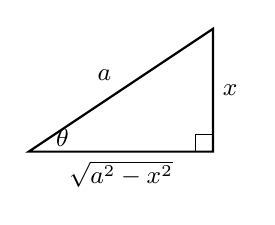
\begin{tikzpicture}[scale=0.78, every node/.style={font=\small}]
  \draw[thick] (0,0) -- (3,0) -- (3,2) -- cycle;
  \draw (2.72,0) -- (2.72,0.28) -- (3,0.28);
  \node at (0.55,0.22) {\(\theta\)};
  \node[below] at (1.5,0) {\(\sqrt{a^2-x^2}\)};
  \node[right] at (3,1) {\(x\)};
  \node[above left] at (1.5,1.0) {\(a\)};
\end{tikzpicture}

\[
\sin\theta=\frac{x}{a}
\]
\end{minipage}
\hfill
\begin{minipage}{0.31\textwidth}
\centering
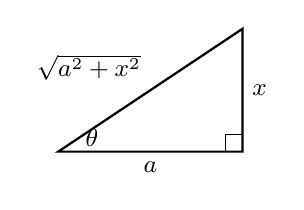
\begin{tikzpicture}[scale=0.78, every node/.style={font=\small}]
  \draw[thick] (0,0) -- (3,0) -- (3,2) -- cycle;
  \draw (2.72,0) -- (2.72,0.28) -- (3,0.28);
  \node at (0.55,0.22) {\(\theta\)};
  \node[below] at (1.5,0) {\(a\)};
  \node[right] at (3,1) {\(x\)};
  \node[above left] at (1.5,1.0) {\(\sqrt{a^2+x^2}\)};
\end{tikzpicture}

\[
\tan\theta=\frac{x}{a}
\]
\end{minipage}
\hfill
\begin{minipage}{0.31\textwidth}
\centering
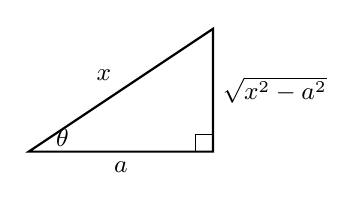
\begin{tikzpicture}[scale=0.78, every node/.style={font=\small}]
  \draw[thick] (0,0) -- (3,0) -- (3,2) -- cycle;
  \draw (2.72,0) -- (2.72,0.28) -- (3,0.28);
  \node at (0.55,0.22) {\(\theta\)};
  \node[below] at (1.5,0) {\(a\)};
  \node[right] at (3,1) {\(\sqrt{x^2-a^2}\)};
  \node[above left] at (1.5,1.0) {\(x\)};
\end{tikzpicture}

\[
\sec\theta=\frac{x}{a}
\]
\end{minipage}
\caption{The three substitutions are right-triangle substitutions.  The triangle helps us return to \(x\).}
\label{fig:trig-substitution-triangles}
\end{figure}

\paragraph{Example: the \(a^2+x^2\) pattern.}
Find

\[
\int \frac{dx}{\sqrt{x^2+4}}.
\]

The expression under the square root has the form

\[
x^2+a^2
\]

with \(a=2\).  Use

\[
x=2\tan\theta.
\]

Then

\[
dx=2\sec^2\theta\,d\theta,
\]

and

\[
\sqrt{x^2+4}
=
\sqrt{4\tan^2\theta+4}
=
2\sqrt{1+\tan^2\theta}
=
2\sec\theta,
\]

where \(\sec\theta>0\) on the chosen interval.

So

\[
\int \frac{dx}{\sqrt{x^2+4}}
=
\int \frac{2\sec^2\theta}{2\sec\theta}\,d\theta
=
\int \sec\theta\,d\theta.
\]

From Section \ref{sec:trigonometric-integrals},

\[
\int \sec\theta\,d\theta
=
\ln|\sec\theta+\tan\theta|+C.
\]

Now return to \(x\).  Since

\[
\tan\theta=\frac{x}{2},
\]

the triangle gives

\[
\sec\theta=\frac{\sqrt{x^2+4}}{2}.
\]

Therefore

\[
\ln|\sec\theta+\tan\theta|
=
\ln\left|\frac{\sqrt{x^2+4}}{2}+\frac{x}{2}\right|.
\]

The factor \(1/2\) inside the logarithm changes the answer only by a constant, so it can
be absorbed into \(C\).  Thus

\[
\boxed{
\int \frac{dx}{\sqrt{x^2+4}}
=
\ln|x+\sqrt{x^2+4}|+C.
}
\]

\paragraph{Example: the \(x^2-a^2\) pattern.}
Find

\[
\int \frac{\sqrt{x^2-4}}{x}\,dx,
\qquad x>2.
\]

The expression under the square root has the form

\[
x^2-a^2
\]

with \(a=2\).  Use

\[
x=2\sec\theta,
\qquad
0\le\theta<\frac{\pi}{2}.
\]

Then

\[
dx=2\sec\theta\tan\theta\,d\theta,
\]

and

\[
\sqrt{x^2-4}
=
\sqrt{4\sec^2\theta-4}
=
2\sqrt{\sec^2\theta-1}
=
2\tan\theta.
\]

The integral becomes

\[
\int
\frac{2\tan\theta}{2\sec\theta}
\cdot
2\sec\theta\tan\theta\,d\theta.
\]

Cancel:

\[
\int \frac{\sqrt{x^2-4}}{x}\,dx
=
2\int \tan^2\theta\,d\theta.
\]

Use

\[
\tan^2\theta=\sec^2\theta-1.
\]

Then

\[
2\int \tan^2\theta\,d\theta
=
2\int(\sec^2\theta-1)\,d\theta.
\]

So

\[
2\int(\sec^2\theta-1)\,d\theta
=
2\tan\theta-2\theta+C.
\]

Now return to \(x\).  Since

\[
x=2\sec\theta,
\]

we have

\[
\sec\theta=\frac{x}{2},
\qquad
\cos\theta=\frac{2}{x}.
\]

Thus

\[
\theta=\arccos\left(\frac{2}{x}\right).
\]

The triangle also gives

\[
\tan\theta=\frac{\sqrt{x^2-4}}{2}.
\]

Therefore

\[
2\tan\theta-2\theta
=
\sqrt{x^2-4}
-
2\arccos\left(\frac{2}{x}\right).
\]

Hence

\[
\boxed{
\int \frac{\sqrt{x^2-4}}{x}\,dx
=
\sqrt{x^2-4}
-
2\arccos\left(\frac{2}{x}\right)
+C,
\qquad x>2.
}
\]

The condition \(x>2\) is not a small detail.  The substitution \(x=2\sec\theta\) with
\(0\le\theta<\pi/2\) covers \(x\ge2\).  On another interval, such as \(x<-2\), we would
choose a different range or adjust the substitution.  Antiderivatives are always local to an
interval where the integrand is defined.

\subsection{Returning to the original variable}
\label{subsec:returning-original-variable}

An indefinite integral should end in the original variable unless the new variable has
been clearly defined.

There are two common ways to return.

\begin{quote}
\textbf{Two ways to return from \(\theta\).}

\begin{center}
\begin{tabular}{c|c}
\textbf{Method} & \textbf{What it does} \\ \hline
Inverse trigonometric function & Uses equations such as \(\theta=\arcsin(x/a)\) or \(\theta=\arctan(x/a)\). \\[5pt]
Right triangle & Uses the substitution to draw a triangle and read \(\sin\theta\), \(\cos\theta\), \(\tan\theta\), or \(\sec\theta\).
\end{tabular}
\end{center}
\end{quote}

In many examples, both methods are needed.  The angle \(\theta\) itself becomes an
inverse trigonometric function.  Other expressions, such as \(\sin2\theta\) or
\(\tan\theta\), are easiest to recover from the triangle.

\paragraph{Definite integrals: change the limits.}
For definite integrals, there is often no need to return to \(x\).  We can change the
limits instead.

Evaluate

\[
\int_0^1 \frac{dx}{\sqrt{4-x^2}}.
\]

Use

\[
x=2\sin\theta.
\]

Then

\[
dx=2\cos\theta\,d\theta,
\]

and

\[
\sqrt{4-x^2}=2\cos\theta
\]

on the chosen range.

Now change the limits.

When

\[
x=0,
\]

we have

\[
0=2\sin\theta,
\]

so

\[
\theta=0.
\]

When

\[
x=1,
\]

we have

\[
1=2\sin\theta,
\]

so

\[
\sin\theta=\frac12,
\qquad
\theta=\frac{\pi}{6}.
\]

Thus

\[
\int_0^1 \frac{dx}{\sqrt{4-x^2}}
=
\int_0^{\pi/6}
\frac{2\cos\theta}{2\cos\theta}\,d\theta.
\]

So

\[
\int_0^1 \frac{dx}{\sqrt{4-x^2}}
=
\int_0^{\pi/6}1\,d\theta
=
\boxed{\frac{\pi}{6}}.
\]

No \(x\)-triangle is needed at the end because the whole calculation stayed in the new
variable after the limits changed.

\begin{quote}
\textbf{A common mistake.}
Do not mix variables in a definite integral.  After substituting \(x=2\sin\theta\), either
change the limits to \(\theta\)-limits or return the antiderivative to \(x\) before evaluating.

The expression

\[
\int_0^1 d\theta
\]

after an \(x\)-substitution is meaningless unless \(0\) and \(1\) have been converted into
the corresponding \(\theta\)-values.
\end{quote}

The differential keeps the direction of the substitution.  If increasing the new variable
moves \(x\) in the opposite direction, the sign of \(dx\) records that reversal.  This is the
same orientation idea we saw in definite integrals.

\subsection{Hyperbolic substitutions}
\label{subsec:hyperbolic-substitutions}

This subsection is optional on a first reading.

Trigonometric substitutions rely on

\[
1+\tan^2\theta=\sec^2\theta
\]

and

\[
\sec^2\theta-1=\tan^2\theta.
\]

There is another pair of functions built for expressions of the form \(x^2+a^2\) and
\(x^2-a^2\).  The hyperbolic sine and cosine are defined by

\[
\sinh u=\frac{e^u-e^{-u}}{2},
\qquad
\cosh u=\frac{e^u+e^{-u}}{2}.
\]

They satisfy

\[
\cosh^2u-\sinh^2u=1.
\]

Their derivatives are

\[
\frac{d}{du}\sinh u=\cosh u,
\qquad
\frac{d}{du}\cosh u=\sinh u.
\]

Because

\[
1+\sinh^2u=\cosh^2u,
\]

the substitution

\[
x=a\sinh u
\]

turns

\[
\sqrt{a^2+x^2}
\]

into

\[
a\cosh u.
\]

Because

\[
\cosh^2u-1=\sinh^2u,
\]

the substitution

\[
x=a\cosh u
\]

turns

\[
\sqrt{x^2-a^2}
\]

into

\[
a\sinh u
\]

when \(x\ge a\).

\paragraph{Example.}
For \(a>0\), find

\[
\int \frac{dx}{\sqrt{x^2+a^2}}.
\]

Use

\[
x=a\sinh u.
\]

Then

\[
dx=a\cosh u\,du,
\]

and

\[
\sqrt{x^2+a^2}
=
\sqrt{a^2\sinh^2u+a^2}
=
a\sqrt{1+\sinh^2u}
=
a\cosh u.
\]

So

\[
\int \frac{dx}{\sqrt{x^2+a^2}}
=
\int \frac{a\cosh u}{a\cosh u}\,du
=
\int 1\,du
=
u+C.
\]

Since

\[
x=a\sinh u,
\]

we have

\[
u=\operatorname{arsinh}\left(\frac{x}{a}\right).
\]

Thus

\[
\boxed{
\int \frac{dx}{\sqrt{x^2+a^2}}
=
\operatorname{arsinh}\left(\frac{x}{a}\right)+C.
}
\]

Using

\[
\operatorname{arsinh} z=\ln\left(z+\sqrt{z^2+1}\right),
\]

this can also be written as

\[
\boxed{
\int \frac{dx}{\sqrt{x^2+a^2}}
=
\ln|x+\sqrt{x^2+a^2}|+C.
}
\]

The hyperbolic substitution gives the logarithmic answer more directly.  It is not a new
kind of calculus.  It is another choice of variable matched to the shape of the square root.

Trigonometric substitution handles square roots by changing the geometry of the
variable.  The next family of integrals has no square roots at all.  It is algebraic: one
polynomial divided by another.  There the right move is not to create a triangle, but to
split one complicated fraction into simpler fractions.

\section{Rational functions and partial fractions}
\label{sec:rational-functions-partial-fractions}

A rational function is a quotient of polynomials:

\[
\frac{P(x)}{Q(x)}.
\]

Some rational functions are easy to integrate.  For example,

\[
\int \frac{dx}{x-3}
=
\ln|x-3|+C,
\]

and

\[
\int \frac{dx}{x^2+1}
=
\arctan x+C.
\]

Partial fractions turns a complicated rational function into a sum of simple ones.  The
method is algebra before calculus.

\[
\boxed{
\text{factor the denominator, split the fraction, then integrate the pieces.}
}
\]

\subsection{Polynomial division}
\label{subsec:polynomial-division-partial-fractions}

Partial fractions begins only after the rational function is \emph{proper}.

\begin{quote}
\textbf{Proper rational function.}
A rational function

\[
\frac{P(x)}{Q(x)}
\]

is called \emph{proper} if

\[
\deg P<\deg Q.
\]
\end{quote}

If the numerator has degree greater than or equal to the denominator, divide first.

\paragraph{Example.}
Find

\[
\int \frac{x^3+1}{x-1}\,dx.
\]

The rational function is not proper because

\[
\deg(x^3+1)=3
\]

and

\[
\deg(x-1)=1.
\]

Divide:

\[
\frac{x^3+1}{x-1}
=
x^2+x+1+\frac{2}{x-1}.
\]

Check:

\[
(x-1)(x^2+x+1)=x^3-1.
\]

So

\[
x^3+1=(x-1)(x^2+x+1)+2.
\]

Now integrate:

\[
\int \frac{x^3+1}{x-1}\,dx
=
\int\left(x^2+x+1+\frac{2}{x-1}\right)\,dx.
\]

Therefore

\[
\boxed{
\int \frac{x^3+1}{x-1}\,dx
=
\frac{x^3}{3}+\frac{x^2}{2}+x+2\ln|x-1|+C.
}
\]

Polynomial division separates the polynomial part from the proper rational part.  Only
the proper part needs partial fractions.

\begin{quote}
\textbf{First move for rational functions.}
Before partial fractions, ask:

\[
\deg P<\deg Q?
\]

If not, divide.
\end{quote}

\subsection{Distinct linear factors}
\label{subsec:distinct-linear-factors}

The simplest partial fractions occur when the denominator factors into distinct linear
factors.

For example,

\[
(x-1)(x+2)
\]

has two different linear factors.  We try to write

\[
\frac{1}{(x-1)(x+2)}
=
\frac{A}{x-1}+\frac{B}{x+2}.
\]

This helps because each piece has a logarithmic antiderivative.

\paragraph{Seed example.}
Find

\[
\int \frac{dx}{(x-1)(x+2)}.
\]

Write

\[
\frac{1}{(x-1)(x+2)}
=
\frac{A}{x-1}+\frac{B}{x+2}.
\]

Multiply both sides by

\[
(x-1)(x+2).
\]

Then

\[
1=A(x+2)+B(x-1).
\]

This identity must hold for all \(x\) in the domain.  Choose values of \(x\) that make
terms disappear.

Set \(x=1\):

\[
1=A(3)+B(0),
\]

so

\[
A=\frac13.
\]

Set \(x=-2\):

\[
1=A(0)+B(-3),
\]

so

\[
B=-\frac13.
\]

Therefore

\[
\frac{1}{(x-1)(x+2)}
=
\frac{1}{3}\frac{1}{x-1}
-
\frac{1}{3}\frac{1}{x+2}.
\]

Now integrate:

\[
\int \frac{dx}{(x-1)(x+2)}
=
\frac13\int\frac{dx}{x-1}
-
\frac13\int\frac{dx}{x+2}.
\]

Thus

\[
\boxed{
\int \frac{dx}{(x-1)(x+2)}
=
\frac13\ln|x-1|
-
\frac13\ln|x+2|
+C.
}
\]

The absolute values belong in the logarithms because \(x-1\) and \(x+2\) can be
positive or negative on different intervals.

\begin{quote}
\textbf{Distinct linear factors.}
If \(P(x)/Q(x)\) is proper and

\[
Q(x)=(x-r_1)(x-r_2)\cdots(x-r_n)
\]

has distinct linear factors, then we try

\[
\frac{P(x)}{Q(x)}
=
\frac{A_1}{x-r_1}
+
\frac{A_2}{x-r_2}
+\cdots+
\frac{A_n}{x-r_n}.
\]
\end{quote}

The constants are found by multiplying by the denominator and comparing the resulting
polynomial identity.

\paragraph{Example.}
Decompose

\[
\frac{3x+5}{(x-2)(x+1)}.
\]

Write

\[
\frac{3x+5}{(x-2)(x+1)}
=
\frac{A}{x-2}+\frac{B}{x+1}.
\]

Multiply by \((x-2)(x+1)\):

\[
3x+5=A(x+1)+B(x-2).
\]

Set \(x=2\):

\[
11=3A,
\]

so

\[
A=\frac{11}{3}.
\]

Set \(x=-1\):

\[
2=-3B,
\]

so

\[
B=-\frac23.
\]

Thus

\[
\frac{3x+5}{(x-2)(x+1)}
=
\frac{11}{3}\frac{1}{x-2}
-
\frac{2}{3}\frac{1}{x+1}.
\]

So

\[
\boxed{
\int \frac{3x+5}{(x-2)(x+1)}\,dx
=
\frac{11}{3}\ln|x-2|
-
\frac{2}{3}\ln|x+1|
+C.
}
\]

\subsection{Repeated linear factors}
\label{subsec:repeated-linear-factors}

If a linear factor is repeated, one fraction is not enough.

For a denominator containing

\[
(x-r)^2,
\]

we need both

\[
\frac{A}{x-r}
\qquad\text{and}\qquad
\frac{B}{(x-r)^2}.
\]

For a denominator containing

\[
(x-r)^3,
\]

we need

\[
\frac{A}{x-r}
+
\frac{B}{(x-r)^2}
+
\frac{C}{(x-r)^3}.
\]

Each power must appear.

\begin{quote}
\textbf{Repeated linear factor.}
A repeated factor

\[
(x-r)^m
\]

contributes

\[
\frac{A_1}{x-r}
+
\frac{A_2}{(x-r)^2}
+\cdots+
\frac{A_m}{(x-r)^m}.
\]
\end{quote}

\paragraph{Example.}
Find

\[
\int \frac{dx}{(x-1)^2(x+2)}.
\]

The denominator contains the repeated factor \((x-1)^2\).  Therefore write

\[
\frac{1}{(x-1)^2(x+2)}
=
\frac{A}{x-1}
+
\frac{B}{(x-1)^2}
+
\frac{C}{x+2}.
\]

Multiply by \((x-1)^2(x+2)\):

\[
1=A(x-1)(x+2)+B(x+2)+C(x-1)^2.
\]

Now choose convenient values.

Set \(x=1\):

\[
1=3B,
\]

so

\[
B=\frac13.
\]

Set \(x=-2\):

\[
1=9C,
\]

so

\[
C=\frac19.
\]

To find \(A\), use any other value, or compare coefficients.  Comparing the coefficient
of \(x^2\),

\[
0=A+C.
\]

Thus

\[
A=-C=-\frac19.
\]

So

\[
\frac{1}{(x-1)^2(x+2)}
=
-\frac{1}{9}\frac{1}{x-1}
+
\frac{1}{3}\frac{1}{(x-1)^2}
+
\frac{1}{9}\frac{1}{x+2}.
\]

Integrate term by term:

\[
\int \frac{dx}{(x-1)^2(x+2)}
=
-\frac19\int\frac{dx}{x-1}
+
\frac13\int\frac{dx}{(x-1)^2}
+
\frac19\int\frac{dx}{x+2}.
\]

Since

\[
\int (x-1)^{-2}\,dx
=
-\frac{1}{x-1},
\]

we get

\[
\boxed{
\int \frac{dx}{(x-1)^2(x+2)}
=
-\frac19\ln|x-1|
-
\frac{1}{3(x-1)}
+
\frac19\ln|x+2|
+C.
}
\]

\begin{quote}
\textbf{Why every power is needed.}
If we tried only

\[
\frac{A}{x-1}+\frac{C}{x+2},
\]

then after multiplying by the denominator we would get

\[
1=A(x-1)(x+2)+C(x-1)^2.
\]

Both terms on the right vanish at \(x=1\), giving \(1=0\).  That is impossible.  The
missing term \(B/(x-1)^2\) is necessary.
\end{quote}

\subsection{Irreducible quadratic factors}
\label{subsec:irreducible-quadratic-factors}

Not every quadratic factors into real linear terms.  For example,

\[
x^2+1
\]

has no real zeros.  It is an \emph{irreducible quadratic factor} over the real numbers.

When such a factor appears, the numerator over it must be linear:

\[
\frac{Bx+C}{x^2+1}.
\]

A constant numerator alone is not enough.  The \(Bx\) part is needed because the
derivative of \(x^2+1\) is \(2x\), and that derivative produces logarithms.

\begin{quote}
\textbf{Irreducible quadratic factor.}
An irreducible quadratic factor

\[
ax^2+bx+c
\]

contributes a partial fraction of the form

\[
\frac{Ax+B}{ax^2+bx+c}.
\]

If the quadratic factor is repeated, include one such numerator over each power.
\end{quote}

\paragraph{Example.}
Find

\[
\int \frac{2x+3}{(x-1)(x^2+1)}\,dx.
\]

The denominator has one linear factor and one irreducible quadratic factor.  Write

\[
\frac{2x+3}{(x-1)(x^2+1)}
=
\frac{A}{x-1}
+
\frac{Bx+C}{x^2+1}.
\]

Multiply both sides by \((x-1)(x^2+1)\):

\[
2x+3=A(x^2+1)+(Bx+C)(x-1).
\]

Expand:

\[
2x+3
=
Ax^2+A+Bx^2-Bx+Cx-C.
\]

Collect terms:

\[
2x+3
=
(A+B)x^2+(-B+C)x+(A-C).
\]

Now match coefficients.

For \(x^2\):

\[
A+B=0.
\]

For \(x\):

\[
-B+C=2.
\]

For the constant term:

\[
A-C=3.
\]

Solving gives

\[
A=\frac52,
\qquad
B=-\frac52,
\qquad
C=-\frac12.
\]

Therefore

\[
\frac{2x+3}{(x-1)(x^2+1)}
=
\frac{5}{2}\frac{1}{x-1}
+
\frac{-\frac52x-\frac12}{x^2+1}.
\]

Now integrate:

\[
\int \frac{2x+3}{(x-1)(x^2+1)}\,dx
=
\frac52\int\frac{dx}{x-1}
-\frac52\int\frac{x}{x^2+1}\,dx
-\frac12\int\frac{dx}{x^2+1}.
\]

The three pieces are

\[
\int\frac{dx}{x-1}=\ln|x-1|,
\]

\[
\int\frac{x}{x^2+1}\,dx=\frac12\ln(x^2+1),
\]

and

\[
\int\frac{dx}{x^2+1}=\arctan x.
\]

Thus

\[
\boxed{
\int \frac{2x+3}{(x-1)(x^2+1)}\,dx
=
\frac52\ln|x-1|
-
\frac54\ln(x^2+1)
-
\frac12\arctan x
+C.
}
\]

The quadratic piece produces two kinds of antiderivatives: a logarithm from the
derivative of the denominator, and an arctangent from the remaining constant part.

\subsection{Completing the square}
\label{subsec:completing-square-partial-fractions}

Quadratic denominators often need one more algebraic step.  Complete the square.

The basic pattern is

\[
x^2+4x+13=(x+2)^2+9.
\]

This turns the denominator into the arctangent form

\[
u^2+a^2.
\]

\paragraph{Example.}
Find

\[
\int \frac{3x+7}{x^2+4x+13}\,dx.
\]

Let

\[
D(x)=x^2+4x+13.
\]

Then

\[
D'(x)=2x+4.
\]

The numerator \(3x+7\) can be split into a multiple of \(D'(x)\) plus a remainder:

\[
3x+7
=
\frac32(2x+4)+1.
\]

Therefore

\[
\int \frac{3x+7}{x^2+4x+13}\,dx
=
\frac32\int \frac{2x+4}{x^2+4x+13}\,dx
+
\int \frac{dx}{x^2+4x+13}.
\]

The first integral is logarithmic:

\[
\frac32\int \frac{2x+4}{x^2+4x+13}\,dx
=
\frac32\ln|x^2+4x+13|.
\]

For the second integral, complete the square:

\[
x^2+4x+13=(x+2)^2+9.
\]

So

\[
\int \frac{dx}{x^2+4x+13}
=
\int\frac{dx}{(x+2)^2+3^2}.
\]

Let

\[
u=x+2.
\]

Then

\[
du=dx,
\]

and

\[
\int\frac{dx}{(x+2)^2+3^2}
=
\int\frac{du}{u^2+3^2}
=
\frac13\arctan\left(\frac{u}{3}\right)+C.
\]

Return to \(x\):

\[
\int \frac{dx}{x^2+4x+13}
=
\frac13\arctan\left(\frac{x+2}{3}\right)+C.
\]

Putting the two parts together gives

\[
\boxed{
\int \frac{3x+7}{x^2+4x+13}\,dx
=
\frac32\ln(x^2+4x+13)
+
\frac13\arctan\left(\frac{x+2}{3}\right)
+C.
}
\]

Here the denominator is always positive, so the absolute value in the logarithm is not
needed.  In the general formula \(\int D'(x)/D(x)\,dx=\ln|D(x)|+C\), the absolute value
is still the safest habit.

\subsection{The partial fractions pattern}
\label{subsec:partial-fractions-pattern}

The method is systematic.

\begin{quote}
\textbf{Partial fractions workflow.}

\begin{center}
\begin{tabular}{c|p{0.72\textwidth}}
\textbf{Step} & \textbf{Action} \\ \hline
1 & If the rational function is not proper, use polynomial division. \\[4pt]
2 & Factor the denominator over the real numbers. \\[4pt]
3 & Write the partial fraction form, including all powers of repeated factors. \\[4pt]
4 & Multiply by the denominator and solve for the constants. \\[4pt]
5 & Integrate the pieces using powers, logarithms, and arctangents.
\end{tabular}
\end{center}
\end{quote}

The building blocks are few.

\[
\int \frac{dx}{x-r}=\ln|x-r|+C,
\]

\[
\int \frac{dx}{(x-r)^m}
=
\frac{(x-r)^{1-m}}{1-m}+C,
\qquad m\neq1,
\]

\[
\int \frac{D'(x)}{D(x)}\,dx=\ln|D(x)|+C,
\]

and

\[
\int \frac{dx}{(x-h)^2+a^2}
=
\frac1a\arctan\left(\frac{x-h}{a}\right)+C.
\]

Partial fractions is not a new antiderivative rule.  It is a way of forcing a rational
function to break into pieces whose antiderivatives we already know.

\paragraph{A final example.}
Find

\[
\int \frac{x^2+2x+4}{x(x+1)^2}\,dx.
\]

The function is proper because the numerator has degree \(2\) and the denominator has
degree \(3\).

The denominator has a distinct factor \(x\) and a repeated factor \((x+1)^2\).  Write

\[
\frac{x^2+2x+4}{x(x+1)^2}
=
\frac{A}{x}
+
\frac{B}{x+1}
+
\frac{C}{(x+1)^2}.
\]

Multiply by \(x(x+1)^2\):

\[
x^2+2x+4
=
A(x+1)^2
+
Bx(x+1)
+
Cx.
\]

Set \(x=0\):

\[
4=A,
\]

so

\[
A=4.
\]

Expand the right side:

\[
4(x+1)^2+Bx(x+1)+Cx.
\]

That is

\[
4(x^2+2x+1)+B(x^2+x)+Cx.
\]

Collect terms:

\[
(4+B)x^2+(8+B+C)x+4.
\]

Match with

\[
x^2+2x+4.
\]

Thus

\[
4+B=1,
\]

so

\[
B=-3.
\]

Also,

\[
8+B+C=2.
\]

Since \(B=-3\),

\[
8-3+C=2,
\]

so

\[
C=-3.
\]

Therefore

\[
\frac{x^2+2x+4}{x(x+1)^2}
=
\frac{4}{x}
-
\frac{3}{x+1}
-
\frac{3}{(x+1)^2}.
\]

Integrate:

\[
\int \frac{x^2+2x+4}{x(x+1)^2}\,dx
=
4\ln|x|
-
3\ln|x+1|
+
\frac{3}{x+1}
+C.
\]

So

\[
\boxed{
\int \frac{x^2+2x+4}{x(x+1)^2}\,dx
=
4\ln|x|
-
3\ln|x+1|
+
\frac{3}{x+1}
+C.
}
\]

We now have several strong methods: substitution, integration by parts, trigonometric
identities, trigonometric substitution, and partial fractions.  The difficult part is no
longer only carrying out a method.  It is choosing the method.  That is the next question.
\section{Strategy for integration}
\label{sec:strategy-for-integration}

We now have several methods:

\[
\text{substitution, integration by parts, trigonometric identities,}
\]

\[
\text{trigonometric substitution, and partial fractions.}
\]

Each method is useful.  None is universal.  The hard part is no longer only carrying out
a technique.  The hard part is recognizing which technique the integral is asking for.

That recognition is not magic.  It comes from looking for structure.

\[
\boxed{
\text{An integration technique is a response to the shape of the integrand.}
}
\]

\subsection{Recognizing the structure of an integrand}
\label{subsec:recognizing-integrand-structure}

A derivative rule leaves a fingerprint.

The chain rule often leaves a function and its derivative:

\[
2x\cos(x^2).
\]

The product rule often leaves a product where one factor becomes simpler when
differentiated:

\[
x e^x,
\qquad
x\ln x,
\qquad
x\cos x.
\]

Trigonometric identities appear when powers of sine, cosine, tangent, or secant are
mixed:

\[
\sin^5x\cos^2x,
\qquad
\tan^3x\sec^4x.
\]

Right-triangle identities appear when a square root has one of the forms

\[
\sqrt{a^2-x^2},
\qquad
\sqrt{a^2+x^2},
\qquad
\sqrt{x^2-a^2}.
\]

Partial fractions appear when the integrand is a rational function:

\[
\frac{P(x)}{Q(x)}.
\]

The first question is therefore not ``What formula do I remember?''  It is:

\[
\boxed{
\text{What structure do I see?}
}
\]

\begin{center}
\begin{tabular}{c|p{0.58\textwidth}}
\textbf{What the integrand looks like} & \textbf{Likely first idea} \\ \hline
A function together with something close to its derivative & Try substitution. \\[5pt]
A product where one factor simplifies when differentiated & Try integration by parts. \\[5pt]
Powers of trigonometric functions & Use trigonometric identities, then substitution. \\[5pt]
A square root like \(a^2-x^2\), \(a^2+x^2\), or \(x^2-a^2\) & Try trigonometric substitution. \\[5pt]
A quotient of polynomials & Use polynomial division if needed, then partial fractions. \\[5pt]
A complicated expression that becomes simpler after expansion, factoring, or rationalizing & Do algebra before choosing a calculus method.
\end{tabular}
\end{center}

This table is a guide, not a law.  Many integrals can be solved in more than one way.
The best method is usually the one that reveals the structure most clearly.

\paragraph{Example: a chain rule fingerprint.}
Find

\[
\int \frac{2x}{1+x^2}\,dx.
\]

The denominator is

\[
1+x^2,
\]

and its derivative is

\[
2x.
\]

That derivative appears in the numerator.  This suggests substitution:

\[
u=1+x^2,
\qquad
du=2x\,dx.
\]

Then

\[
\int \frac{2x}{1+x^2}\,dx
=
\int \frac{du}{u}
=
\ln|u|+C.
\]

So

\[
\boxed{
\int \frac{2x}{1+x^2}\,dx
=
\ln(1+x^2)+C.
}
\]

The absolute value is not needed in the final expression because

\[
1+x^2>0
\]

for all real \(x\).

\paragraph{Example: a product rule fingerprint.}
Find

\[
\int x e^x\,dx.
\]

There is no inside function whose derivative appears.  But the integrand is a product,
and the factor \(x\) becomes simpler when differentiated.  So use integration by parts:

\[
u=x,
\qquad
dv=e^x\,dx.
\]

Then

\[
du=dx,
\qquad
v=e^x.
\]

Thus

\[
\int x e^x\,dx
=
xe^x-\int e^x\,dx.
\]

Therefore

\[
\boxed{
\int x e^x\,dx=xe^x-e^x+C.
}
\]

\paragraph{Example: a rational function fingerprint.}
Find

\[
\int \frac{x+5}{x^2-x-6}\,dx.
\]

The integrand is a rational function.  Factor the denominator:

\[
x^2-x-6=(x-3)(x+2).
\]

Use partial fractions:

\[
\frac{x+5}{(x-3)(x+2)}
=
\frac{A}{x-3}+\frac{B}{x+2}.
\]

Multiply by \((x-3)(x+2)\):

\[
x+5=A(x+2)+B(x-3).
\]

Set \(x=3\):

\[
8=5A,
\qquad
A=\frac85.
\]

Set \(x=-2\):

\[
3=-5B,
\qquad
B=-\frac35.
\]

So

\[
\frac{x+5}{x^2-x-6}
=
\frac{8}{5}\frac{1}{x-3}
-
\frac{3}{5}\frac{1}{x+2}.
\]

Therefore

\[
\boxed{
\int \frac{x+5}{x^2-x-6}\,dx
=
\frac85\ln|x-3|-\frac35\ln|x+2|+C.
}
\]

The structure chose the method.

\subsection{Substitution first or parts first?}
\label{subsec:substitution-first-or-parts-first}

Some integrals look like products but are really substitution problems.  Others look like
they might have an inside function, but integration by parts is better.

A useful test is this:

\[
\boxed{
\text{Before using parts, check whether substitution removes the whole problem.}
}
\]

Integration by parts creates a new integral.  Substitution often turns the integral directly
into a known form.  So substitution is usually the first thing to test.

\paragraph{Example: a product that is really substitution.}
Find

\[
\int x e^{x^2}\,dx.
\]

The integrand is a product, but the exponent has inside function

\[
x^2,
\]

whose derivative is

\[
2x.
\]

So substitution is the natural choice:

\[
u=x^2,
\qquad
du=2x\,dx.
\]

Then

\[
x\,dx=\frac12\,du.
\]

Therefore

\[
\int x e^{x^2}\,dx
=
\frac12\int e^u\,du
=
\frac12 e^u+C.
\]

So

\[
\boxed{
\int x e^{x^2}\,dx
=
\frac12 e^{x^2}+C.
}
\]

Trying integration by parts would make this worse.  The product is not the main
structure.  The inside function \(x^2\) is.

\paragraph{Example: a product that really needs parts.}
Find

\[
\int x e^x\,dx.
\]

Here the exponent is just \(x\).  Its derivative is \(1\), not a missing factor that simplifies
the integral.  Substitution does not help.

But \(x\) becomes simpler when differentiated, and \(e^x\) is easy to integrate.  So
integration by parts gives

\[
\int x e^x\,dx=xe^x-e^x+C.
\]

The two examples are close in appearance:

\[
\int x e^{x^2}\,dx
\qquad\text{and}\qquad
\int x e^x\,dx.
\]

But their structures are different.  The first is a chain rule problem.  The second is a
product rule problem.

\paragraph{Example: logarithms often want parts.}
Find

\[
\int x\ln x\,dx,
\qquad x>0.
\]

There is no helpful substitution.  The factor \(\ln x\) becomes simpler when
differentiated:

\[
\frac{d}{dx}\ln x=\frac1x.
\]

Choose

\[
u=\ln x,
\qquad
dv=x\,dx.
\]

Then

\[
du=\frac1x\,dx,
\qquad
v=\frac{x^2}{2}.
\]

Integration by parts gives

\[
\int x\ln x\,dx
=
\frac{x^2}{2}\ln x-\int \frac{x^2}{2}\cdot \frac1x\,dx.
\]

So

\[
\int x\ln x\,dx
=
\frac{x^2}{2}\ln x-\frac12\int x\,dx.
\]

Therefore

\[
\boxed{
\int x\ln x\,dx
=
\frac{x^2}{2}\ln x-\frac{x^2}{4}+C.
}
\]

A logarithm is often a good choice for \(u\), because it simplifies under
differentiation.

\begin{quote}
\textbf{Substitution or parts?}

Substitution asks:

\[
\text{Is there an inside function whose derivative is present?}
\]

Integration by parts asks:

\[
\text{Can I differentiate one factor and make it simpler, while integrating the other factor?}
\]

When both seem possible, try substitution first.  If it does not simplify the integral,
look for parts.
\end{quote}

\subsection{Algebraic simplification}
\label{subsec:algebraic-simplification-before-integration}

Sometimes the right technique is hidden behind algebra.  Before reaching for a new
calculus method, simplify the integrand.

Algebra can reveal substitution, partial fractions, cancellation, or a known form.

\paragraph{Example: divide before integrating.}
Find

\[
\int \frac{x^2-1}{x-1}\,dx.
\]

The expression looks rational, but the numerator factors:

\[
x^2-1=(x-1)(x+1).
\]

For \(x\neq1\),

\[
\frac{x^2-1}{x-1}=x+1.
\]

Therefore

\[
\int \frac{x^2-1}{x-1}\,dx
=
\int (x+1)\,dx.
\]

So

\[
\boxed{
\int \frac{x^2-1}{x-1}\,dx
=
\frac{x^2}{2}+x+C,
\qquad x\neq1.
}
\]

The original integrand is not defined at \(x=1\).  An indefinite integral is always
understood on an interval in the domain, such as \((-\infty,1)\) or \((1,\infty)\).

\paragraph{Example: shift before expanding.}
Find

\[
\int x\sqrt{x+1}\,dx.
\]

This could tempt us toward integration by parts.  But the square root suggests the
substitution

\[
u=x+1.
\]

Then

\[
x=u-1,
\qquad
dx=du.
\]

The integral becomes

\[
\int (u-1)\sqrt{u}\,du.
\]

Now simplify:

\[
(u-1)\sqrt{u}=u^{3/2}-u^{1/2}.
\]

So

\[
\int (u^{3/2}-u^{1/2})\,du
=
\frac{2}{5}u^{5/2}-\frac{2}{3}u^{3/2}+C.
\]

Return to \(x\):

\[
\boxed{
\int x\sqrt{x+1}\,dx
=
\frac{2}{5}(x+1)^{5/2}
-
\frac{2}{3}(x+1)^{3/2}
+C.
}
\]

The substitution did not immediately give a basic antiderivative.  It gave an algebraic
expression we could simplify.

\paragraph{Example: rationalizing can reveal a simple form.}
Find

\[
\int \frac{dx}{\sqrt{x+1}+\sqrt{x}}.
\]

At first this does not match any standard pattern.  Multiply numerator and denominator
by the conjugate:

\[
\frac{1}{\sqrt{x+1}+\sqrt{x}}
\cdot
\frac{\sqrt{x+1}-\sqrt{x}}{\sqrt{x+1}-\sqrt{x}}.
\]

The denominator becomes

\[
(x+1)-x=1.
\]

So

\[
\frac{1}{\sqrt{x+1}+\sqrt{x}}
=
\sqrt{x+1}-\sqrt{x}.
\]

Therefore

\[
\int \frac{dx}{\sqrt{x+1}+\sqrt{x}}
=
\int \bigl(\sqrt{x+1}-\sqrt{x}\bigr)\,dx.
\]

Now integrate term by term:

\[
\int \sqrt{x+1}\,dx
=
\frac23(x+1)^{3/2},
\]

and

\[
\int \sqrt{x}\,dx
=
\frac23x^{3/2}.
\]

Thus

\[
\boxed{
\int \frac{dx}{\sqrt{x+1}+\sqrt{x}}
=
\frac23(x+1)^{3/2}
-
\frac23x^{3/2}
+C.
}
\]

The calculus was easy after the algebra.

\begin{quote}
\textbf{Algebra before technique.}
Before choosing an integration method, ask whether the integrand can be simplified by

\[
\text{factoring, canceling, expanding, completing the square,}
\]

\[
\text{dividing polynomials, using identities, or rationalizing.}
\]

A hard-looking integral may become a basic one after the right algebraic move.
\end{quote}

\subsection{A practical decision tree}
\label{subsec:integration-decision-tree}

No decision tree can replace judgment.  But a rough order helps.

\begin{figure}[h]
\centering
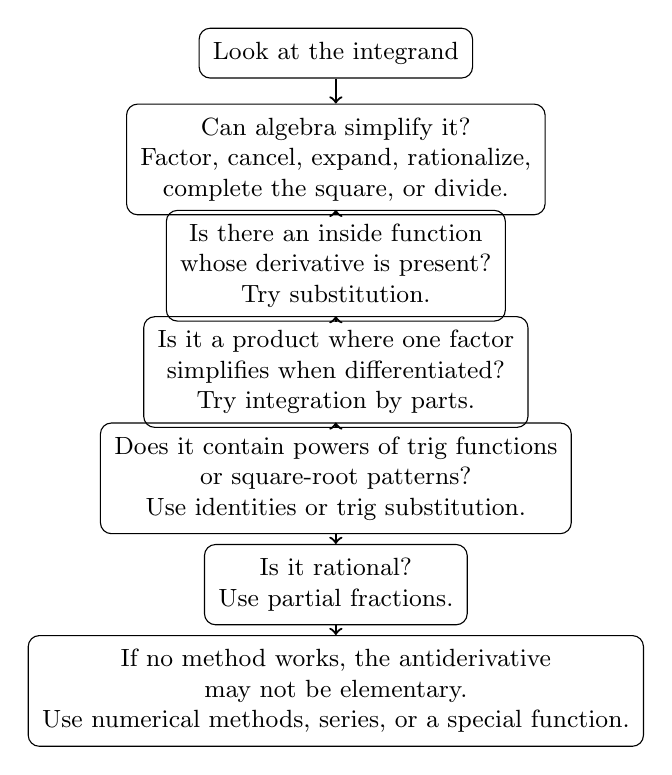
\begin{tikzpicture}[
  node distance=1.35cm,
  box/.style={draw, rounded corners, align=center, inner sep=5pt, font=\small},
  arrow/.style={->, thick}
]
\node[box] (start) {Look at the integrand};
\node[box, below of=start] (algebra) {Can algebra simplify it?\\Factor, cancel, expand, rationalize,\\complete the square, or divide.};
\node[box, below of=algebra] (sub) {Is there an inside function\\whose derivative is present?\\Try substitution.};
\node[box, below of=sub] (parts) {Is it a product where one factor\\simplifies when differentiated?\\Try integration by parts.};
\node[box, below of=parts] (trig) {Does it contain powers of trig functions\\or square-root patterns?\\Use identities or trig substitution.};
\node[box, below of=trig] (rat) {Is it rational?\\Use partial fractions.};
\node[box, below of=rat] (none) {If no method works, the antiderivative\\may not be elementary.\\Use numerical methods, series, or a special function.};

\draw[arrow] (start) -- (algebra);
\draw[arrow] (algebra) -- (sub);
\draw[arrow] (sub) -- (parts);
\draw[arrow] (parts) -- (trig);
\draw[arrow] (trig) -- (rat);
\draw[arrow] (rat) -- (none);
\end{tikzpicture}
\caption{A practical order of questions.  The arrows are not laws; they are a way to begin thinking.}
\label{fig:integration-decision-tree}
\end{figure}

The order matters less than the habit: pause, read the integrand, and identify the
structure.

\paragraph{Example: a mixed decision.}
Find

\[
\int \frac{x^3}{\sqrt{x^2+1}}\,dx.
\]

The square root suggests a possible trigonometric substitution, but there is also an
inside function:

\[
x^2+1.
\]

Its derivative is \(2x\), and the numerator contains \(x^3\,dx\).  Rewrite

\[
x^3\,dx=x^2(x\,dx).
\]

Use

\[
u=x^2+1,
\qquad
du=2x\,dx.
\]

Then

\[
x\,dx=\frac12\,du,
\]

and

\[
x^2=u-1.
\]

The integral becomes

\[
\int \frac{x^3}{\sqrt{x^2+1}}\,dx
=
\frac12\int \frac{u-1}{\sqrt{u}}\,du.
\]

Simplify:

\[
\frac{u-1}{\sqrt u}=u^{1/2}-u^{-1/2}.
\]

So

\[
\frac12\int \left(u^{1/2}-u^{-1/2}\right)\,du
=
\frac12\left(\frac23u^{3/2}-2u^{1/2}\right)+C.
\]

Thus

\[
\frac12\int \left(u^{1/2}-u^{-1/2}\right)\,du
=
\frac13u^{3/2}-u^{1/2}+C.
\]

Return to \(x\):

\[
\boxed{
\int \frac{x^3}{\sqrt{x^2+1}}\,dx
=
\frac13(x^2+1)^{3/2}
-
(x^2+1)^{1/2}
+C.
}
\]

A trigonometric substitution would work, but it would be longer.  The simpler inside
function was already present.

\paragraph{Example: a definite integral can simplify by symmetry.}
Evaluate

\[
\int_{-2}^{2} x e^{-x^2}\,dx.
\]

The integrand

\[
x e^{-x^2}
\]

is odd, because

\[
(-x)e^{-(-x)^2}=-xe^{-x^2}.
\]

The interval \([-2,2]\) is symmetric about \(0\).  Therefore the positive and negative
parts cancel:

\[
\boxed{
\int_{-2}^{2} x e^{-x^2}\,dx=0.
}
\]

We could also use substitution, but symmetry is faster and more revealing.

\begin{quote}
\textbf{For definite integrals, use definite information.}
Before finding an antiderivative, check for

\[
\text{symmetry, sign, cancellation, geometry, and bounds.}
\]

A definite integral may have a simple value even when the indefinite integral is hard.
\end{quote}

\subsection{When no elementary antiderivative exists}
\label{subsec:no-elementary-antiderivative}

It is natural to hope that every continuous function has a familiar antiderivative.
The Fundamental Theorem tells us that every continuous function \(f\) has an
antiderivative:

\[
F(x)=\int_a^x f(t)\,dt.
\]

But it does not say that \(F\) can be written using the elementary functions we already
know.

By \emph{elementary functions}, we mean functions built from polynomials, rational
functions, powers, exponentials, logarithms, trigonometric functions, inverse
trigonometric functions, and combinations of these by addition, subtraction,
multiplication, division, and composition.

Many elementary functions have antiderivatives that are not elementary.

Famous examples include

\[
\int e^{-x^2}\,dx,
\]

\[
\int \frac{\sin x}{x}\,dx,
\]

\[
\int \sin(x^2)\,dx,
\]

and

\[
\int \frac{dx}{\ln x}.
\]

This is not a failure of calculus.  It is a sign that the family of elementary functions is
not closed under antidifferentiation.

\paragraph{The Gaussian example.}
The function

\[
e^{-x^2}
\]

is continuous everywhere.  Therefore

\[
G(x)=\int_0^x e^{-t^2}\,dt
\]

is a perfectly good function, and the Fundamental Theorem gives

\[
G'(x)=e^{-x^2}.
\]

But \(G(x)\) cannot be expressed using elementary functions.  So instead of forcing it
into old language, mathematicians name it.  A scaled version is called the error function:

\[
\operatorname{erf}(x)
=
\frac{2}{\sqrt{\pi}}\int_0^x e^{-t^2}\,dt.
\]

The name is not a trick.  It is a recognition that this accumulation is important enough
to become a function in its own right.

\paragraph{A definite integral may still be meaningful.}
Even if

\[
\int e^{-x^2}\,dx
\]

has no elementary antiderivative, the definite integral

\[
\int_0^1 e^{-x^2}\,dx
\]

still has a definite value.  It measures accumulated area.  We can approximate it
numerically.  Later, we will also approximate it with power series.

The absence of an elementary antiderivative does not stop the integral from existing.

\[
\boxed{
\text{Exact elementary formulas are useful, but they are not the only way to know an integral.}
}
\]

\subsection{Strategy summary}
\label{subsec:strategy-summary}

Integration is less mechanical than differentiation.  Differentiation has a direct rule for
each way of building a function.  Integration asks us to recognize what construction
might have produced the integrand.

A useful final checklist is:

\begin{center}
\begin{tabular}{c|p{0.62\textwidth}}
\textbf{Question} & \textbf{Possible response} \\ \hline
Can the integrand be simplified algebraically? & Factor, cancel, expand, rationalize, complete the square, or divide. \\[5pt]
Is there an inside function with its derivative nearby? & Use substitution. \\[5pt]
Is there a product with a factor that simplifies under differentiation? & Use integration by parts. \\[5pt]
Are there trigonometric powers or products? & Use identities and then substitute. \\[5pt]
Is there a square root matching a Pythagorean pattern? & Use trigonometric or hyperbolic substitution. \\[5pt]
Is the integrand rational? & Use polynomial division and partial fractions. \\[5pt]
Is it a definite integral with symmetry or geometry? & Use the bounds and the shape before seeking an antiderivative. \\[5pt]
Does no elementary method work? & Define a new accumulation function, approximate numerically, or use series.
\end{tabular}
\end{center}

The best way to learn strategy is to practice with mixed examples.  But the guiding
principle stays simple:

\[
\boxed{
\text{Do not ask first, ``What technique should I use?''}
}
\]

Ask instead:

\[
\boxed{
\text{What is the integrand trying to tell me?}
}
\]

The next section adds a modern tool.  Computer algebra systems and integral tables can
find many antiderivatives.  But they do not remove the need for thought.  They make
checking, interpretation, and domain awareness more important.

\section{Computer algebra systems and integral tables}
\label{sec:cas-and-integral-tables}

A computer algebra system can differentiate, integrate, simplify, factor, expand, and
solve equations.  An integral table can list thousands of antiderivative patterns.

These tools are useful.  They are also dangerous when used passively.

A tool may give an answer that is correct on one interval but not another.  It may return
an expression that looks different from yours.  It may use a special function you have not
seen before.  It may hide an absolute value.  It may even produce a form that is harder to
understand than the original problem.

So the rule is:

\[
\boxed{
\text{Use tools to check and explore, not to surrender judgment.}
}
\]

\subsection{Checking without surrendering thought}
\label{subsec:checking-without-surrendering-thought}

The simplest way to check an antiderivative is to differentiate it.

If a tool says

\[
\int f(x)\,dx=F(x)+C,
\]

then check whether

\[
F'(x)=f(x).
\]

This works no matter how complicated \(F\) looks.

\paragraph{Example.}
Suppose a table or computer gives

\[
\int x\cos(x^2)\,dx=\frac12\sin(x^2)+C.
\]

Check by differentiating:

\[
\frac{d}{dx}\left(\frac12\sin(x^2)\right)
=
\frac12\cos(x^2)\cdot 2x
=
x\cos(x^2).
\]

The derivative matches the integrand, so the answer is correct.

Notice what the check also teaches.  The integral came from substitution:

\[
u=x^2,
\qquad
du=2x\,dx.
\]

A good tool answer should make the structure more visible after we inspect it.

\paragraph{Example: checking a table formula.}
A table may list

\[
\int e^{ax}\cos(bx)\,dx
=
\frac{e^{ax}}{a^2+b^2}\bigl(a\cos bx+b\sin bx\bigr)+C.
\]

Use it to find

\[
\int e^{2x}\cos(3x)\,dx.
\]

Here

\[
a=2,
\qquad
b=3.
\]

So

\[
\int e^{2x}\cos(3x)\,dx
=
\frac{e^{2x}}{2^2+3^2}\bigl(2\cos 3x+3\sin 3x\bigr)+C.
\]

Thus

\[
\boxed{
\int e^{2x}\cos(3x)\,dx
=
\frac{e^{2x}}{13}\bigl(2\cos 3x+3\sin 3x\bigr)+C.
}
\]

A table formula should still be checked.  Differentiate

\[
F(x)=\frac{e^{2x}}{13}\bigl(2\cos 3x+3\sin 3x\bigr).
\]

Using the product rule,

\[
F'(x)
=
\frac{e^{2x}}{13}\cdot 2\bigl(2\cos 3x+3\sin 3x\bigr)
+
\frac{e^{2x}}{13}\bigl(-6\sin 3x+9\cos 3x\bigr).
\]

Collect terms:

\[
F'(x)
=
\frac{e^{2x}}{13}
\bigl(4\cos 3x+6\sin 3x-6\sin 3x+9\cos 3x\bigr).
\]

So

\[
F'(x)
=
\frac{e^{2x}}{13}(13\cos 3x)
=
e^{2x}\cos 3x.
\]

The check confirms the formula.

\begin{quote}
\textbf{How to use a table or CAS answer.}

\begin{center}
\begin{tabular}{c|p{0.66\textwidth}}
\textbf{Step} & \textbf{Question} \\ \hline
1 & Does the answer differentiate back to the integrand? \\[4pt]
2 & On what interval is the formula valid? \\[4pt]
3 & Are absolute values needed in logarithms? \\[4pt]
4 & Is the answer equivalent to a simpler form? \\[4pt]
5 & Does the definite integral require checking endpoints or discontinuities?
\end{tabular}
\end{center}
\end{quote}

The derivative check is powerful, but it does not answer every question.  Domains and
branches still matter.

\subsection{Equivalent antiderivatives can look different}
\label{subsec:equivalent-antiderivatives}

Two correct antiderivatives of the same function may look different.  If they differ only
by a constant on an interval, they represent the same family of antiderivatives.

\[
F'(x)=G'(x)
\quad\Longrightarrow\quad
F(x)-G(x)=\text{constant}
\]

on any interval where both functions are differentiable.

\paragraph{Example: two forms for \(\int \tan x\,dx\).}
One method gives

\[
\int \tan x\,dx
=
-\ln|\cos x|+C.
\]

Another form is

\[
\int \tan x\,dx
=
\ln|\sec x|+C.
\]

These are the same because

\[
\sec x=\frac1{\cos x}.
\]

Therefore

\[
\ln|\sec x|
=
\ln\left|\frac1{\cos x}\right|
=
-\ln|\cos x|.
\]

So

\[
\boxed{
-\ln|\cos x|
\quad\text{and}\quad
\ln|\sec x|
}
\]

are equivalent antiderivatives.

\paragraph{Example: partial fractions can be written in one logarithm.}
From partial fractions,

\[
\int \frac{dx}{x^2-1}
=
\frac12\ln|x-1|-\frac12\ln|x+1|+C.
\]

Using logarithm rules,

\[
\frac12\ln|x-1|-\frac12\ln|x+1|
=
\frac12\ln\left|\frac{x-1}{x+1}\right|.
\]

So an equivalent answer is

\[
\boxed{
\int \frac{dx}{x^2-1}
=
\frac12\ln\left|\frac{x-1}{x+1}\right|+C.
}
\]

A computer may give either form.  A table may give another equivalent form.  The
right response is not to panic, but to differentiate or simplify.

\paragraph{Example: inverse trigonometric forms can differ.}
Consider

\[
\int \frac{dx}{\sqrt{1-x^2}}.
\]

One antiderivative is

\[
\arcsin x+C.
\]

Another is

\[
-\arccos x+C.
\]

They are equivalent because

\[
\frac{d}{dx}\arcsin x=\frac1{\sqrt{1-x^2}},
\]

and

\[
\frac{d}{dx}\bigl(-\arccos x\bigr)
=
-\left(-\frac1{\sqrt{1-x^2}}\right)
=
\frac1{\sqrt{1-x^2}}.
\]

In fact,

\[
\arcsin x+\arccos x=\frac{\pi}{2}
\]

for \(-1\le x\le1\), so the two antiderivatives differ by a constant:

\[
\arcsin x
=
-\arccos x+\frac{\pi}{2}.
\]

The same derivative can wear different costumes.

\begin{quote}
\textbf{Equivalent answers.}
If your answer and a tool's answer look different, compare them by

\[
\text{simplifying, using identities, or differentiating their difference.}
\]

If the difference is constant on the interval, both answers are correct.
\end{quote}

\subsection{Branch and domain issues}
\label{subsec:branch-domain-issues}

An indefinite integral is not a global object on every part of the real line at once.  It is
usually a family of antiderivatives on intervals where the integrand is defined.

This matters most for logarithms, square roots, and inverse trigonometric functions.

\paragraph{Example: the missing absolute value.}
A computer system might return

\[
\ln x
\]

for

\[
\int \frac{dx}{x}.
\]

That is correct on the interval

\[
(0,\infty).
\]

But in real calculus, the function \(1/x\) is also defined on

\[
(-\infty,0).
\]

On that interval, an antiderivative is

\[
\ln(-x),
\]

because

\[
\frac{d}{dx}\ln(-x)=\frac1{-x}\cdot(-1)=\frac1x.
\]

The compact real formula is

\[
\boxed{
\int \frac{dx}{x}=\ln|x|+C.
}
\]

The absolute value combines the two intervals into one notation.

But the domain is still split.  The integrand is not defined at \(x=0\), and no
antiderivative crosses through \(0\).

\paragraph{Example: logarithms from substitution.}
Find

\[
\int \frac{x}{x^2-1}\,dx.
\]

Use

\[
u=x^2-1,
\qquad
du=2x\,dx.
\]

Then

\[
\int \frac{x}{x^2-1}\,dx
=
\frac12\int \frac{du}{u}
=
\frac12\ln|u|+C.
\]

So

\[
\boxed{
\int \frac{x}{x^2-1}\,dx
=
\frac12\ln|x^2-1|+C.
}
\]

A tool may return

\[
\frac12\ln(x^2-1).
\]

That expression is real only where

\[
x^2-1>0,
\]

which means

\[
x<-1
\qquad\text{or}\qquad
x>1.
\]

But the original integrand is also defined on

\[
(-1,1),
\]

where

\[
x^2-1<0.
\]

On that interval, the real antiderivative needs

\[
\ln|x^2-1|.
\]

The absolute value is not decoration.  It preserves the real antiderivative on every
interval where the integrand is defined.

\paragraph{Example: square-root domains.}
The antiderivative

\[
\int \frac{dx}{\sqrt{1-x^2}}
=
\arcsin x+C
\]

is a real formula on

\[
-1<x<1.
\]

The integrand itself requires

\[
1-x^2>0,
\]

so the natural open interval is \((-1,1)\).  At \(x=\pm1\), the denominator is zero.

When a tool returns an inverse trigonometric expression, always ask:

\[
\text{On what interval is the original integrand real and finite?}
\]

and

\[
\text{Which branch of the inverse trigonometric function is being used?}
\]

In a first calculus course, we usually choose the standard branches:

\[
-\frac{\pi}{2}\le \arcsin x\le \frac{\pi}{2},
\]

\[
0\le \arccos x\le \pi,
\]

\[
-\frac{\pi}{2}<\arctan x<\frac{\pi}{2}.
\]

Those choices make inverse trigonometric functions into genuine functions.  They also
control the signs that appear when returning from a trigonometric substitution.

\begin{quote}
\textbf{Domain warning.}
A symbolic answer may be correct only on part of the domain.  For real-valued calculus,
always check

\[
\text{zeros of denominators, signs inside square roots,}
\]

\[
\text{absolute values in logarithms, and inverse-function branches.}
\]
\end{quote}

\subsection{Integral tables}
\label{subsec:integral-tables}

Before computer algebra systems, students and scientists used integral tables.  A table is
not only a list of answers.  It is a catalog of patterns.

For example, a table may list

\[
\int \frac{du}{a^2+u^2}
=
\frac1a\arctan\left(\frac{u}{a}\right)+C,
\qquad a>0.
\]

To use the table, we must match the pattern.

\paragraph{Example.}
Find

\[
\int \frac{dx}{9+(2x-1)^2}.
\]

The denominator has the form

\[
a^2+u^2
\]

with

\[
a=3,
\qquad
u=2x-1.
\]

But the numerator is \(dx\), while the table formula wants \(du\).  Since

\[
du=2\,dx,
\]

we have

\[
dx=\frac12\,du.
\]

Therefore

\[
\int \frac{dx}{9+(2x-1)^2}
=
\frac12\int \frac{du}{9+u^2}.
\]

Using the table formula with \(a=3\),

\[
\frac12\int \frac{du}{9+u^2}
=
\frac12\cdot\frac13\arctan\left(\frac{u}{3}\right)+C.
\]

So

\[
\boxed{
\int \frac{dx}{9+(2x-1)^2}
=
\frac16\arctan\left(\frac{2x-1}{3}\right)+C.
}
\]

The table did not replace substitution.  It worked together with substitution.

\paragraph{Example: a table formula with a square root.}
A table may list

\[
\int \sqrt{a^2-u^2}\,du
=
\frac{u}{2}\sqrt{a^2-u^2}
+
\frac{a^2}{2}\arcsin\left(\frac{u}{a}\right)
+C.
\]

Use it to find

\[
\int \sqrt{25-4x^2}\,dx.
\]

Rewrite the square root as

\[
\sqrt{25-(2x)^2}.
\]

Let

\[
u=2x,
\qquad
du=2\,dx,
\qquad
dx=\frac12\,du.
\]

Then

\[
\int \sqrt{25-4x^2}\,dx
=
\frac12\int \sqrt{25-u^2}\,du.
\]

Here \(a=5\).  Apply the formula:

\[
\frac12\left[
\frac{u}{2}\sqrt{25-u^2}
+
\frac{25}{2}\arcsin\left(\frac{u}{5}\right)
\right]+C.
\]

So

\[
\int \sqrt{25-4x^2}\,dx
=
\frac{u}{4}\sqrt{25-u^2}
+
\frac{25}{4}\arcsin\left(\frac{u}{5}\right)
+C.
\]

Return to \(x\):

\[
\boxed{
\int \sqrt{25-4x^2}\,dx
=
\frac{x}{2}\sqrt{25-4x^2}
+
\frac{25}{4}\arcsin\left(\frac{2x}{5}\right)
+C.
}
\]

The factor \(1/2\) from \(du=2\,dx\) is the kind of detail that tables do not manage for
us.  We must manage the change of variable.

\subsection{Special functions born from integrals}
\label{subsec:special-functions-born-from-integrals}

When an elementary antiderivative does not exist, we do not abandon the integral.
We define a new function by accumulation.

This has already happened in ordinary calculus.  The natural logarithm can be defined by

\[
\ln x=\int_1^x \frac{dt}{t},
\qquad x>0.
\]

So a function born from an integral is not strange.  It is one of the oldest ideas in the
subject.

\paragraph{The error function.}
The function

\[
e^{-x^2}
\]

has no elementary antiderivative.  But the accumulation

\[
\int_0^x e^{-t^2}\,dt
\]

is important in probability and statistics.  A standard scaled version is

\[
\boxed{
\operatorname{erf}(x)=\frac{2}{\sqrt{\pi}}\int_0^x e^{-t^2}\,dt.
}
\]

By the Fundamental Theorem,

\[
\operatorname{erf}'(x)
=
\frac{2}{\sqrt{\pi}}e^{-x^2}.
\]

So the derivative is completely clear, even though the function is not elementary.

\paragraph{The sine integral.}
Another important example is

\[
\boxed{
\operatorname{Si}(x)=\int_0^x \frac{\sin t}{t}\,dt.
}
\]

The integrand appears to have a problem at \(t=0\), but

\[
\lim_{t\to0}\frac{\sin t}{t}=1.
\]

So we define the integrand at \(0\) by its limiting value \(1\).  Then the accumulation
makes sense.

For \(x\neq0\),

\[
\operatorname{Si}'(x)=\frac{\sin x}{x}.
\]

With the continuous extension at \(x=0\),

\[
\operatorname{Si}'(0)=1.
\]

Special functions are not failures.  They are named accumulations that occur often
enough to deserve their own notation.

\begin{quote}
\textbf{A new function is sometimes the honest answer.}
If

\[
F(x)=\int_a^x f(t)\,dt
\]

cannot be written with elementary functions, \(F\) is still a function.  It can be
graphed, approximated, differentiated, tabulated, and used in models.
\end{quote}

\subsection{Definite integrals and symbolic answers}
\label{subsec:definite-integrals-symbolic-answers}

A computer algebra system may return a special function for a definite integral.  That is
not necessarily less useful than a decimal.

For example,

\[
\int_0^1 e^{-x^2}\,dx
\]

can be written as

\[
\frac{\sqrt{\pi}}{2}\operatorname{erf}(1).
\]

This is an exact expression in terms of a special function.  A decimal approximation is
also useful:

\[
\int_0^1 e^{-x^2}\,dx\approx0.7468.
\]

The exact form and the decimal form answer different needs.

\begin{center}
\begin{tabular}{c|p{0.55\textwidth}}
\textbf{Form} & \textbf{What it is good for} \\ \hline
Exact elementary expression & Algebraic manipulation, exact comparison, symbolic work. \\[4pt]
Special-function expression & Exact naming of a non-elementary accumulation. \\[4pt]
Decimal approximation & Measurement, computation, practical estimation.
\end{tabular}
\end{center}

The important question is not always ``Can we find an elementary antiderivative?''  Often
the better question is:

\[
\text{How accurately do we need the accumulated amount?}
\]

That question leads naturally to numerical integration.

\subsection{A responsible workflow with tools}
\label{subsec:responsible-workflow-tools}

When using a table or computer algebra system, work in this order.

\begin{quote}
\textbf{Responsible use of symbolic integration.}

\begin{center}
\begin{tabular}{c|p{0.70\textwidth}}
\textbf{Step} & \textbf{Action} \\ \hline
1 & Inspect the integrand first.  Identify possible structure. \\[4pt]
2 & Try a human method if the structure is clear. \\[4pt]
3 & Use a table or CAS to check, compare, or explore. \\[4pt]
4 & Differentiate the returned antiderivative. \\[4pt]
5 & Check the interval, branch, and absolute values. \\[4pt]
6 & For a definite integral, check whether endpoints or discontinuities cause trouble. \\[4pt]
7 & Decide whether an exact form, special-function form, or decimal approximation is most useful.
\end{tabular}
\end{center}
\end{quote}

The last endpoint check points toward the next section.  A definite integral over a finite
interval with a continuous integrand is safe.  But many important integrals are not of that
kind.  The interval may be infinite.  The integrand may blow up.  A formal antiderivative
may exist while the accumulated amount is not finite.

For example,

\[
\int_1^\infty \frac{dx}{x}
\]

has the antiderivative

\[
\ln x,
\]

but the accumulated area grows without bound.

So the next question is not how to find an antiderivative.  It is more basic:

\[
\boxed{
\text{When does an infinite or singular accumulation have a finite value?}
}
\]

That is the problem of improper integrals.\Computing
\section{Improper integrals}
\label{sec:improper-integrals}

The last section ended with a warning.  A definite integral over a closed, finite interval is
safe when the integrand is continuous.  The interval has finite length, the function stays
bounded, and the accumulated amount is a finite number.

But many natural accumulations do not fit that safe pattern.

A radioactive particle may decay forever.  A probability density may stretch over the
whole real line.  A force law may blow up near a point.  A curve may enclose an infinite
region whose area is still finite.

So we have to ask a more careful question:

\[
\boxed{
\text{When does an infinite or singular accumulation have a finite value?}
}
\]

That is the question of improper integrals.

An improper integral is not wrong or badly formed.  The word \emph{improper} means
that the integral lies outside the original definition and must be interpreted as a limit.

\subsection{Infinite intervals}
\label{subsec:infinite-intervals}

Start with an infinite interval.

The expression

\[
\int_1^\infty \frac{1}{x^2}\,dx
\]

asks for the area under \(1/x^2\) from \(x=1\) onward forever.  We cannot add area all
the way to infinity in one step.  Instead, we stop at a finite number \(t\), compute

\[
\int_1^t \frac{1}{x^2}\,dx,
\]

and then let \(t\) move farther and farther to the right.

For \(t>1\),

\[
\int_1^t \frac{1}{x^2}\,dx
=
\int_1^t x^{-2}\,dx
=
\left[-\frac1x\right]_1^t
=
-\frac1t+1.
\]

Now let \(t\to\infty\):

\[
\lim_{t\to\infty}\left(1-\frac1t\right)=1.
\]

Therefore

\[
\boxed{
\int_1^\infty \frac{1}{x^2}\,dx=1.
}
\]

This infinite region has finite area.

Now compare

\[
\int_1^\infty \frac1x\,dx.
\]

Again stop at \(t\):

\[
\int_1^t \frac1x\,dx
=
\ln x\Big|_1^t
=
\ln t.
\]

As \(t\to\infty\),

\[
\ln t\to\infty.
\]

So

\[
\boxed{
\int_1^\infty \frac1x\,dx
\text{ diverges.}
}
\]

Both functions

\[
\frac1x
\qquad\text{and}\qquad
\frac1{x^2}
\]

approach \(0\).  But only \(1/x^2\) approaches \(0\) fast enough to have finite total
area on the infinite interval.

\begin{figure}[h]
\centering
\begin{minipage}{0.47\textwidth}
\centering
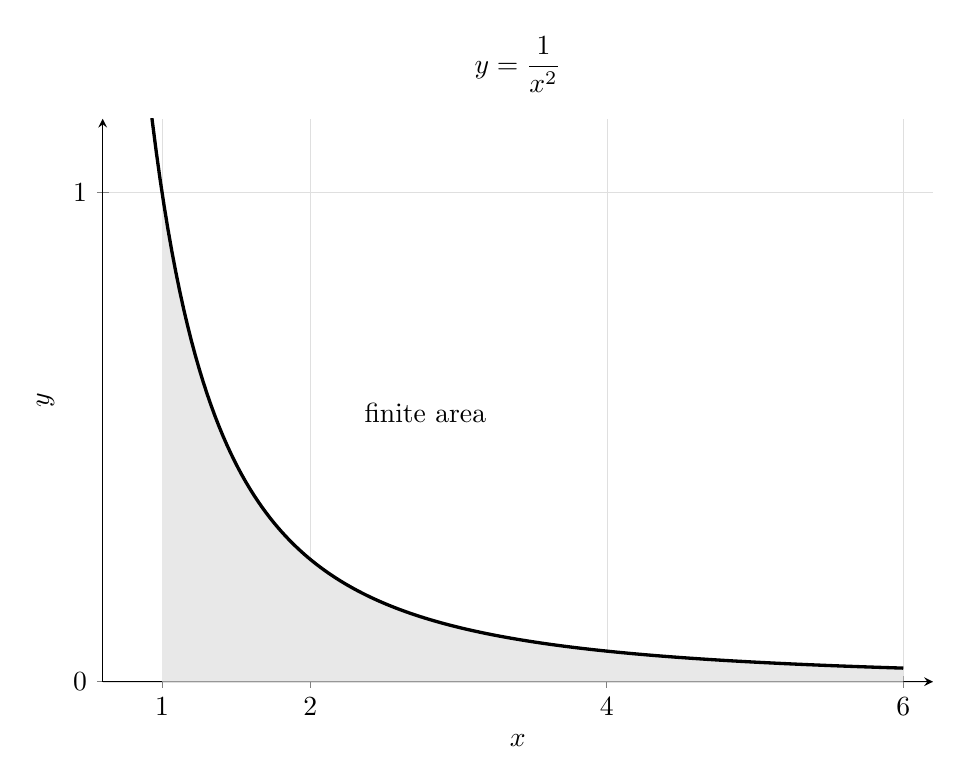
\begin{tikzpicture}
\begin{axis}[
    width=\textwidth,
    height=0.72\textwidth,
    xmin=0.6, xmax=6.2,
    ymin=0, ymax=1.15,
    axis lines=left,
    xlabel={\(x\)},
    ylabel={\(y\)},
    xtick={1,2,4,6},
    ytick={0,1},
    grid=both,
    grid style={line width=.1pt, draw=gray!25},
    title={\(\displaystyle y=\frac1{x^2}\)}
]
\addplot[domain=1:6, samples=150, fill=gray!18, draw=none] {1/(x^2)} \closedcycle;
\addplot[very thick, domain=0.75:6, samples=200] {1/(x^2)};
\node[anchor=west] at (axis cs:2.3,0.55) {finite area};
\end{axis}
\end{tikzpicture}
\end{minipage}
\hfill
\begin{minipage}{0.47\textwidth}
\centering
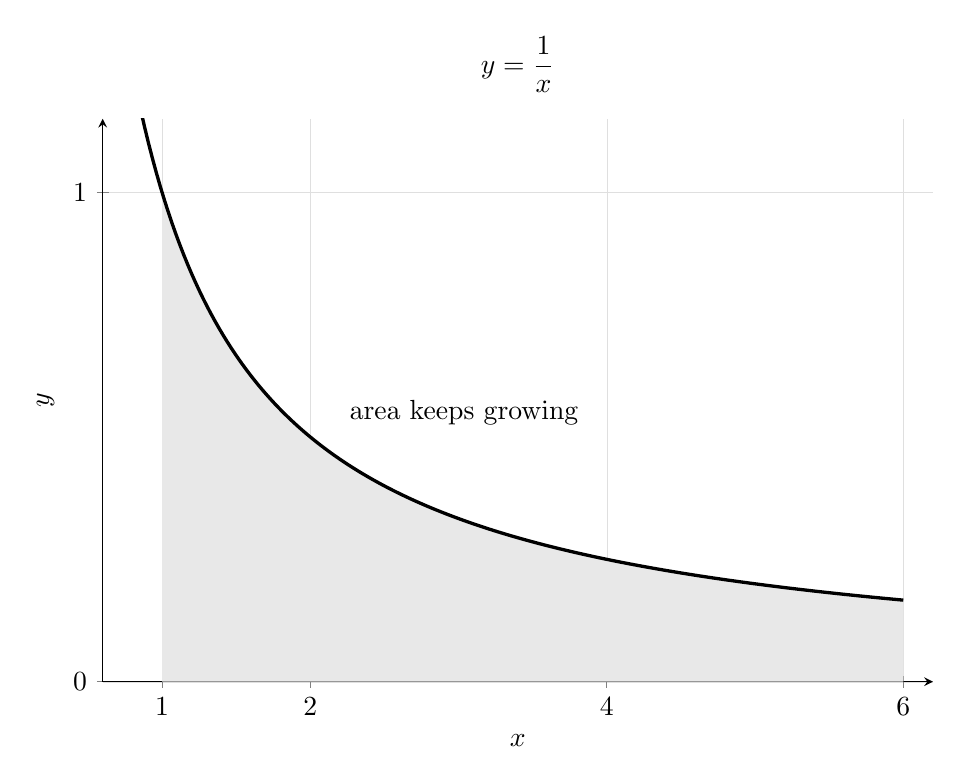
\begin{tikzpicture}
\begin{axis}[
    width=\textwidth,
    height=0.72\textwidth,
    xmin=0.6, xmax=6.2,
    ymin=0, ymax=1.15,
    axis lines=left,
    xlabel={\(x\)},
    ylabel={\(y\)},
    xtick={1,2,4,6},
    ytick={0,1},
    grid=both,
    grid style={line width=.1pt, draw=gray!25},
    title={\(\displaystyle y=\frac1x\)}
]
\addplot[domain=1:6, samples=150, fill=gray!18, draw=none] {1/x} \closedcycle;
\addplot[very thick, domain=0.75:6, samples=200] {1/x};
\node[anchor=west] at (axis cs:2.2,0.55) {area keeps growing};
\end{axis}
\end{tikzpicture}
\end{minipage}
\caption{Both curves approach \(0\), but the tail of \(1/x\) has infinite area while the tail of \(1/x^2\) has finite area.}
\label{fig:one-over-x-vs-one-over-x-squared}
\end{figure}

This example motivates the definition.

\begin{quote}
\textbf{Improper integral on an infinite interval.}
If \(f\) is continuous on \([a,t]\) for every \(t>a\), then

\[
\boxed{
\int_a^\infty f(x)\,dx
=
\lim_{t\to\infty}\int_a^t f(x)\,dx
}
\]

provided the limit exists as a finite number.

If the limit exists as a finite number, the improper integral \emph{converges}.  If the
limit does not exist as a finite number, the improper integral \emph{diverges}.
\end{quote}

Similarly,

\[
\boxed{
\int_{-\infty}^b f(x)\,dx
=
\lim_{t\to-\infty}\int_t^b f(x)\,dx
}
\]

provided the limit exists as a finite number.

For an integral over the whole real line, split at any convenient point \(c\):

\[
\boxed{
\int_{-\infty}^{\infty} f(x)\,dx
=
\int_{-\infty}^{c} f(x)\,dx
+
\int_c^{\infty} f(x)\,dx.
}
\]

Both pieces must converge.  If either piece diverges, then the whole improper integral
diverges.

\paragraph{Example: an infinite interval in both directions.}
Evaluate

\[
\int_{-\infty}^{\infty} \frac{1}{1+x^2}\,dx.
\]

Split at \(0\):

\[
\int_{-\infty}^{\infty} \frac{1}{1+x^2}\,dx
=
\int_{-\infty}^{0} \frac{1}{1+x^2}\,dx
+
\int_0^{\infty} \frac{1}{1+x^2}\,dx.
\]

For the right half,

\[
\int_0^\infty \frac{1}{1+x^2}\,dx
=
\lim_{t\to\infty}\int_0^t \frac{1}{1+x^2}\,dx.
\]

Since

\[
\int \frac{1}{1+x^2}\,dx=\arctan x+C,
\]

we get

\[
\int_0^\infty \frac{1}{1+x^2}\,dx
=
\lim_{t\to\infty}\bigl(\arctan t-\arctan 0\bigr)
=
\frac{\pi}{2}.
\]

For the left half,

\[
\int_{-\infty}^0 \frac{1}{1+x^2}\,dx
=
\lim_{t\to-\infty}\int_t^0 \frac{1}{1+x^2}\,dx.
\]

Thus

\[
\int_{-\infty}^0 \frac{1}{1+x^2}\,dx
=
\lim_{t\to-\infty}\bigl(\arctan 0-\arctan t\bigr)
=
\frac{\pi}{2}.
\]

Therefore

\[
\boxed{
\int_{-\infty}^{\infty} \frac{1}{1+x^2}\,dx=\pi.
}
\]

This integral appears in probability.  It is also a reminder that finite area can stretch
across an infinite line.

\subsection{Infinite discontinuities}
\label{subsec:infinite-discontinuities}

The interval can be finite and the integral can still be improper.

Consider

\[
\int_0^1 \frac{1}{\sqrt{x}}\,dx.
\]

The interval \([0,1]\) is finite, but the integrand is not defined at \(x=0\), and

\[
\frac{1}{\sqrt{x}}\to\infty
\qquad\text{as}\qquad
x\to0^+.
\]

So we approach the endpoint by a limit:

\[
\int_0^1 \frac{1}{\sqrt{x}}\,dx
=
\lim_{t\to0^+}\int_t^1 \frac{1}{\sqrt{x}}\,dx.
\]

Compute:

\[
\int_t^1 x^{-1/2}\,dx
=
\left[2\sqrt{x}\right]_t^1
=
2-2\sqrt{t}.
\]

Let \(t\to0^+\):

\[
\lim_{t\to0^+}(2-2\sqrt{t})=2.
\]

Therefore

\[
\boxed{
\int_0^1 \frac{1}{\sqrt{x}}\,dx=2.
}
\]

The graph shoots upward near \(0\), but the spike is narrow enough to have finite area.

Now compare

\[
\int_0^1 \frac1x\,dx.
\]

Again,

\[
\int_0^1 \frac1x\,dx
=
\lim_{t\to0^+}\int_t^1 \frac1x\,dx.
\]

For \(0<t<1\),

\[
\int_t^1 \frac1x\,dx
=
\left[\ln x\right]_t^1
=
-\ln t.
\]

As \(t\to0^+\),

\[
-\ln t\to\infty.
\]

So

\[
\boxed{
\int_0^1 \frac1x\,dx
\text{ diverges.}
}
\]

\begin{figure}[h]
\centering
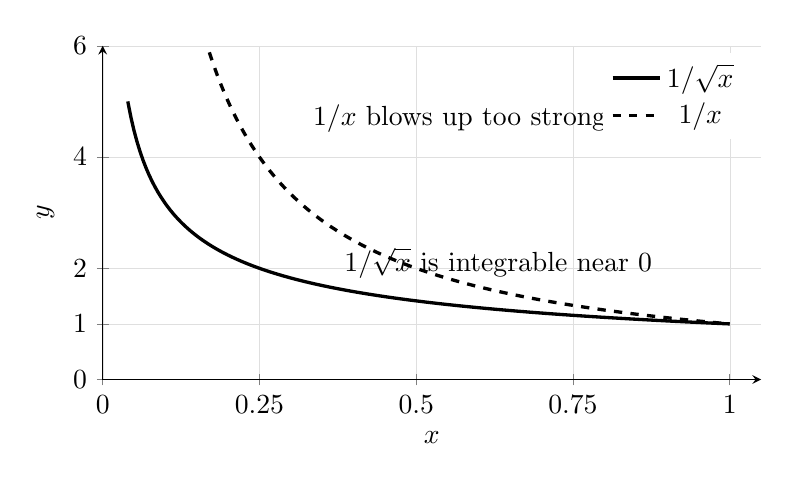
\begin{tikzpicture}
\begin{axis}[
    width=0.82\textwidth,
    height=0.48\textwidth,
    xmin=0, xmax=1.05,
    ymin=0, ymax=6,
    axis lines=left,
    xlabel={\(x\)},
    ylabel={\(y\)},
    xtick={0,0.25,0.5,0.75,1},
    ytick={0,1,2,4,6},
    grid=both,
    grid style={line width=.1pt, draw=gray!25},
    legend style={draw=none, at={(0.98,0.98)}, anchor=north east}
]
\addplot[very thick, domain=0.04:1, samples=200] {1/sqrt(x)};
\addlegendentry{\(\displaystyle 1/\sqrt{x}\)}
\addplot[very thick, dashed, domain=0.17:1, samples=200] {1/x};
\addlegendentry{\(\displaystyle 1/x\)}
\node[anchor=west] at (axis cs:0.32,4.7) {\(\displaystyle 1/x\) blows up too strongly};
\node[anchor=west] at (axis cs:0.37,2.1) {\(\displaystyle 1/\sqrt{x}\) is integrable near \(0\)};
\end{axis}
\end{tikzpicture}
\caption{A function may become infinite near an endpoint and still have finite area.  The rate of blowup matters.}
\label{fig:infinite-discontinuity-comparison}
\end{figure}

\begin{quote}
\textbf{Improper integral with an infinite endpoint discontinuity.}
If \(f\) is continuous on \((a,b]\), but has an infinite discontinuity at \(a\), then

\[
\boxed{
\int_a^b f(x)\,dx
=
\lim_{t\to a^+}\int_t^b f(x)\,dx
}
\]

provided the limit exists as a finite number.

If \(f\) is continuous on \([a,b)\), but has an infinite discontinuity at \(b\), then

\[
\boxed{
\int_a^b f(x)\,dx
=
\lim_{t\to b^-}\int_a^t f(x)\,dx.
}
\]
\end{quote}

If the infinite discontinuity occurs at an interior point \(c\), split the integral:

\[
\boxed{
\int_a^b f(x)\,dx
=
\int_a^c f(x)\,dx+\int_c^b f(x)\,dx.
}
\]

Both pieces must converge.  If either one diverges, the original integral diverges.

\paragraph{Example: a singularity inside the interval.}
Decide whether

\[
\int_{-1}^{1} \frac{1}{\sqrt{|x|}}\,dx
\]

converges.

The integrand is singular at \(x=0\).  Split there:

\[
\int_{-1}^{1} \frac{1}{\sqrt{|x|}}\,dx
=
\int_{-1}^{0} \frac{1}{\sqrt{|x|}}\,dx
+
\int_0^{1} \frac{1}{\sqrt{|x|}}\,dx.
\]

On \((0,1]\),

\[
\frac{1}{\sqrt{|x|}}=\frac1{\sqrt{x}},
\]

so

\[
\int_0^1 \frac{1}{\sqrt{|x|}}\,dx=2.
\]

On \([-1,0)\), use the substitution \(u=-x\).  Then \(du=-dx\), and

\[
\int_{-1}^{0} \frac{1}{\sqrt{|x|}}\,dx
=
\int_1^0 \frac{1}{\sqrt{u}}(-du)
=
\int_0^1 \frac{1}{\sqrt{u}}\,du
=
2.
\]

Both pieces converge, so the original integral converges and

\[
\boxed{
\int_{-1}^{1} \frac{1}{\sqrt{|x|}}\,dx=4.
}
\]

\subsection{Convergence and divergence}
\label{subsec:convergence-divergence-improper}

The words \emph{convergent} and \emph{divergent} describe the limiting process, not the
antiderivative.

An improper integral converges if the limiting accumulated amount approaches a finite
number.  It diverges if the limiting accumulated amount does not approach a finite
number.

\[
\boxed{
\text{convergent means finite accumulated amount.}
}
\]

\[
\boxed{
\text{divergent means no finite accumulated amount.}
}
\]

The antiderivative may exist on every finite subinterval and the improper integral may
still diverge.

For example,

\[
\int_1^t \frac1x\,dx=\ln t
\]

exists for every finite \(t>1\).  But

\[
\lim_{t\to\infty}\ln t=\infty.
\]

So

\[
\int_1^\infty \frac1x\,dx
\]

diverges.

\paragraph{Example: exponential decay.}
Evaluate

\[
\int_0^\infty e^{-x}\,dx.
\]

By definition,

\[
\int_0^\infty e^{-x}\,dx
=
\lim_{t\to\infty}\int_0^t e^{-x}\,dx.
\]

Now

\[
\int_0^t e^{-x}\,dx
=
\left[-e^{-x}\right]_0^t
=
1-e^{-t}.
\]

As \(t\to\infty\),

\[
e^{-t}\to0.
\]

Therefore

\[
\boxed{
\int_0^\infty e^{-x}\,dx=1.
}
\]

Exponential decay wins easily against an infinite interval.

\paragraph{Example: a mean waiting time.}
Evaluate

\[
\int_0^\infty x e^{-x}\,dx.
\]

Stop at \(t\):

\[
\int_0^\infty x e^{-x}\,dx
=
\lim_{t\to\infty}\int_0^t x e^{-x}\,dx.
\]

Use integration by parts on the finite integral.  Let

\[
u=x,
\qquad
dv=e^{-x}\,dx.
\]

Then

\[
du=dx,
\qquad
v=-e^{-x}.
\]

So

\[
\int_0^t x e^{-x}\,dx
=
\left[-xe^{-x}\right]_0^t+\int_0^t e^{-x}\,dx.
\]

This gives

\[
\int_0^t x e^{-x}\,dx
=
-te^{-t}+1-e^{-t}.
\]

Now let \(t\to\infty\).  We know

\[
e^{-t}\to0
\]

and

\[
te^{-t}\to0.
\]

Therefore

\[
\boxed{
\int_0^\infty x e^{-x}\,dx=1.
}
\]

This integral appears as an expected value for an exponential waiting-time model.  The
calculus statement is simple: the tail decays fast enough that the total weighted area is
finite.

\subsection{Comparison tests for improper integrals}
\label{subsec:comparison-tests-improper-integrals}

Many improper integrals cannot be evaluated exactly.  But convergence is often easier
than exact value.

For example,

\[
\int_1^\infty e^{-x^2}\,dx
\]

has no elementary antiderivative.  Still, it converges.  For \(x\ge1\),

\[
x^2\ge x,
\]

so

\[
e^{-x^2}\le e^{-x}.
\]

Since

\[
\int_1^\infty e^{-x}\,dx
\]

converges, the smaller nonnegative function \(e^{-x^2}\) also has finite area.

This is the comparison idea.

\begin{quote}
\textbf{Direct Comparison Test for improper integrals.}
Suppose

\[
0\le f(x)\le g(x)
\]

for all sufficiently large \(x\).

If

\[
\int_a^\infty g(x)\,dx
\]

converges, then

\[
\int_a^\infty f(x)\,dx
\]

also converges.

If

\[
0\le g(x)\le f(x)
\]

for all sufficiently large \(x\), and

\[
\int_a^\infty g(x)\,dx
\]

diverges, then

\[
\int_a^\infty f(x)\,dx
\]

also diverges.
\end{quote}

The phrase ``for all sufficiently large \(x\)'' means that the comparison only needs to
hold eventually.  A finite beginning of the interval cannot decide whether an infinite
tail has finite area.

\paragraph{Example: convergence without an antiderivative.}
Show that

\[
\int_1^\infty e^{-x^2}\,dx
\]

converges.

For \(x\ge1\),

\[
x^2\ge x.
\]

Multiplying by \(-1\) reverses the inequality:

\[
-x^2\le -x.
\]

Since the exponential function is increasing,

\[
e^{-x^2}\le e^{-x}.
\]

Also,

\[
0\le e^{-x^2}.
\]

We know

\[
\int_1^\infty e^{-x}\,dx=e^{-1},
\]

so the comparison test gives

\[
\boxed{
\int_1^\infty e^{-x^2}\,dx
\text{ converges.}
}
\]

We have proved convergence without finding an elementary antiderivative.

\paragraph{Example: divergence by comparison.}
Show that

\[
\int_1^\infty \frac{1+\cos^2 x}{x}\,dx
\]

diverges.

Since

\[
\cos^2x\ge0,
\]

we have

\[
1+\cos^2x\ge1.
\]

Therefore

\[
\frac{1+\cos^2x}{x}\ge\frac1x
\]

for \(x\ge1\).

But

\[
\int_1^\infty \frac1x\,dx
\]

diverges.  The integrand is nonnegative and at least as large as a divergent tail.
Therefore

\[
\boxed{
\int_1^\infty \frac{1+\cos^2 x}{x}\,dx
\text{ diverges.}
}
\]

Comparison needs nonnegative functions.  If signs cancel, the situation is more delicate.
The warning examples in the next section show why.

\begin{quote}
\textbf{Limit Comparison Test for improper integrals.}
Suppose \(f(x)>0\) and \(g(x)>0\) for all sufficiently large \(x\).  If

\[
\lim_{x\to\infty}\frac{f(x)}{g(x)}=L
\]

where

\[
0<L<\infty,
\]

then

\[
\int_a^\infty f(x)\,dx
\]

and

\[
\int_a^\infty g(x)\,dx
\]

either both converge or both diverge.
\end{quote}

The reason is that, far out in the tail, \(f\) behaves like a constant multiple of \(g\).  A
constant multiple changes the size of the area, but not whether the total area is finite.

\paragraph{Example: a rational tail.}
Determine whether

\[
\int_1^\infty \frac{3x^2+1}{x^3+5}\,dx
\]

converges or diverges.

For large \(x\), the integrand behaves like

\[
\frac{3x^2}{x^3}=\frac3x.
\]

Use limit comparison with

\[
g(x)=\frac1x.
\]

Compute

\[
\lim_{x\to\infty}
\frac{\frac{3x^2+1}{x^3+5}}{\frac1x}
=
\lim_{x\to\infty}
\frac{x(3x^2+1)}{x^3+5}.
\]

The highest powers dominate:

\[
\lim_{x\to\infty}
\frac{3x^3+x}{x^3+5}
=
3.
\]

Since

\[
0<3<\infty
\]

and

\[
\int_1^\infty \frac1x\,dx
\]

diverges, the given integral also diverges:

\[
\boxed{
\int_1^\infty \frac{3x^2+1}{x^3+5}\,dx
\text{ diverges.}
}
\]

\paragraph{Example: a convergent rational tail.}
Determine whether

\[
\int_1^\infty \frac{2x+1}{x^3+4}\,dx
\]

converges.

For large \(x\),

\[
\frac{2x+1}{x^3+4}
\sim
\frac{2x}{x^3}
=
\frac2{x^2}.
\]

Use limit comparison with

\[
g(x)=\frac1{x^2}.
\]

Then

\[
\lim_{x\to\infty}
\frac{\frac{2x+1}{x^3+4}}{\frac1{x^2}}
=
\lim_{x\to\infty}
\frac{x^2(2x+1)}{x^3+4}
=
2.
\]

Since

\[
\int_1^\infty \frac1{x^2}\,dx
\]

converges, the given integral converges:

\[
\boxed{
\int_1^\infty \frac{2x+1}{x^3+4}\,dx
\text{ converges.}
}
\]

\subsection{The \texorpdfstring{\(p\)-integrals}{p-integrals}}
\label{subsec:p-integrals}

The most useful comparison family is

\[
\frac1{x^p}.
\]

The power \(p\) decides whether the tail is thin enough.

First consider the infinite interval:

\[
\int_1^\infty \frac1{x^p}\,dx.
\]

If \(p\neq1\), then

\[
\int_1^t x^{-p}\,dx
=
\left[\frac{x^{1-p}}{1-p}\right]_1^t
=
\frac{t^{1-p}-1}{1-p}.
\]

If \(p>1\), then \(1-p<0\), so

\[
t^{1-p}\to0
\qquad\text{as}\qquad
t\to\infty.
\]

The integral converges, and

\[
\int_1^\infty \frac1{x^p}\,dx
=
\frac1{p-1}.
\]

If \(p<1\), then \(1-p>0\), so

\[
t^{1-p}\to\infty.
\]

The integral diverges.

If \(p=1\), then

\[
\int_1^\infty \frac1x\,dx
\]

diverges logarithmically.

Thus

\[
\boxed{
\int_1^\infty \frac1{x^p}\,dx
\text{ converges exactly when } p>1.
}
\]

Now consider the endpoint singularity:

\[
\int_0^1 \frac1{x^p}\,dx.
\]

If \(p\neq1\), then

\[
\int_t^1 x^{-p}\,dx
=
\left[\frac{x^{1-p}}{1-p}\right]_t^1
=
\frac{1-t^{1-p}}{1-p}.
\]

If \(p<1\), then \(1-p>0\), so

\[
t^{1-p}\to0
\qquad\text{as}\qquad
t\to0^+.
\]

The integral converges, and

\[
\int_0^1 \frac1{x^p}\,dx
=
\frac1{1-p}.
\]

If \(p>1\), then \(1-p<0\), so \(t^{1-p}\to\infty\), and the integral diverges.

If \(p=1\), then

\[
\int_0^1 \frac1x\,dx
\]

also diverges.

Thus

\[
\boxed{
\int_0^1 \frac1{x^p}\,dx
\text{ converges exactly when } p<1.
}
\]

\begin{center}
\begin{tabular}{c|c|c}
\textbf{Integral} & \textbf{Converges when} & \textbf{Diverges when} \\ \hline
\(\displaystyle \int_1^\infty \frac1{x^p}\,dx\) & \(p>1\) & \(p\le1\) \\[8pt]
\(\displaystyle \int_0^1 \frac1{x^p}\,dx\) & \(p<1\) & \(p\ge1\)
\end{tabular}
\end{center}

The two thresholds point in opposite directions because the danger is different.

On

\[
[1,\infty),
\]

the danger is the infinite length of the interval.  We need the function to decay faster
than \(1/x\).

On

\[
(0,1],
\]

the danger is the blowup at \(0\).  We need the blowup to be milder than \(1/x\).

\paragraph{Example.}
Determine whether

\[
\int_2^\infty \frac{1}{x\sqrt{x}}\,dx
\]

converges.

Rewrite the integrand:

\[
\frac{1}{x\sqrt{x}}
=
\frac1{x^{3/2}}.
\]

This is a \(p\)-integral with

\[
p=\frac32.
\]

Since

\[
\frac32>1,
\]

the integral converges.

\paragraph{Example.}
Determine whether

\[
\int_0^1 \frac{1}{x^{4/3}}\,dx
\]

converges.

This is a \(p\)-integral near \(0\) with

\[
p=\frac43.
\]

Since

\[
\frac43\ge1,
\]

the integral diverges.

\paragraph{Example: comparison with a \(p\)-integral.}
Determine whether

\[
\int_1^\infty \frac{dx}{x^2+\sqrt{x}}
\]

converges.

For \(x\ge1\),

\[
x^2+\sqrt{x}\ge x^2.
\]

Therefore

\[
0\le \frac{1}{x^2+\sqrt{x}}\le \frac1{x^2}.
\]

Since

\[
\int_1^\infty \frac1{x^2}\,dx
\]

converges, the comparison test gives

\[
\boxed{
\int_1^\infty \frac{dx}{x^2+\sqrt{x}}
\text{ converges.}
}
\]

The exact value is not needed.  We only need enough information to know that the
tail has finite accumulated area.

Improper integrals teach a useful discipline.  Do not evaluate first and ask questions
later.  First ask where the integral is improper.  Then replace the dangerous endpoint
or discontinuity by a limit.  Then decide whether the limit is finite.

The next section collects the mistakes this discipline prevents.

\section{Warning examples}
\label{sec:warning-examples-improper-integrals}

Improper integrals are limits.  That one sentence prevents many errors.

The errors below are common because they look like ordinary applications of the
Fundamental Theorem of Calculus.  But the Fundamental Theorem applies directly only
on intervals where the integrand is continuous.  When the interval is infinite or the
integrand blows up, the limit must be handled first.

\subsection{An antiderivative exists formally but the improper integral diverges}
\label{subsec:formal-antiderivative-improper-diverges}

Consider

\[
\int_{-1}^{1}\frac1{x^2}\,dx.
\]

A tempting but wrong computation is

\[
\int_{-1}^{1}\frac1{x^2}\,dx
=
\left[-\frac1x\right]_{-1}^{1}
=
-1-1
=
-2.
\]

This cannot be right.  The integrand

\[
\frac1{x^2}
\]

is positive wherever it is defined, so its area cannot be negative.

The error is that \(1/x^2\) is not continuous on \([-1,1]\).  It has an infinite
discontinuity at \(x=0\).  We must split the integral:

\[
\int_{-1}^{1}\frac1{x^2}\,dx
=
\int_{-1}^{0}\frac1{x^2}\,dx
+
\int_{0}^{1}\frac1{x^2}\,dx.
\]

Now examine the right-hand piece:

\[
\int_0^1 \frac1{x^2}\,dx
=
\lim_{t\to0^+}\int_t^1 x^{-2}\,dx.
\]

Compute:

\[
\int_t^1 x^{-2}\,dx
=
\left[-\frac1x\right]_t^1
=
-1+\frac1t.
\]

As \(t\to0^+\),

\[
-1+\frac1t\to\infty.
\]

So

\[
\int_0^1 \frac1{x^2}\,dx
\]

diverges.  Therefore

\[
\boxed{
\int_{-1}^{1}\frac1{x^2}\,dx
\text{ diverges.}
}
\]

The antiderivative \(-1/x\) is valid on each interval where \(x\neq0\).  It is not a
license to jump across \(x=0\).

\begin{quote}
\textbf{Moral.}
Before using

\[
\int_a^b f(x)\,dx=F(b)-F(a),
\]

check that \(f\) is continuous on the interval.  If not, split the interval and use limits.
\end{quote}

\subsection{Cancellation hides divergence}
\label{subsec:cancellation-hides-divergence}

Some divergent improper integrals look harmless because positive and negative parts
cancel symmetrically.

Consider

\[
\int_{-1}^{1}\frac1x\,dx.
\]

The graph of \(1/x\) is negative on \((-1,0)\) and positive on \((0,1)\).  If we cut out a
symmetric gap around \(0\), then

\[
\int_{-1}^{-\varepsilon}\frac1x\,dx
+
\int_{\varepsilon}^{1}\frac1x\,dx
=
0.
\]

So one might think the integral is \(0\).

But that is not the definition of the improper integral.  Because the singularity is at
\(0\), we must split:

\[
\int_{-1}^{1}\frac1x\,dx
=
\int_{-1}^{0}\frac1x\,dx
+
\int_0^1\frac1x\,dx.
\]

The right-hand piece is

\[
\int_0^1 \frac1x\,dx
=
\lim_{t\to0^+}\int_t^1 \frac1x\,dx
=
\lim_{t\to0^+}\bigl(0-\ln t\bigr)
=
\infty.
\]

The left-hand piece is

\[
\int_{-1}^{0} \frac1x\,dx
=
\lim_{t\to0^-}\int_{-1}^{t} \frac1x\,dx
=
\lim_{t\to0^-}\ln|t|
=
-\infty.
\]

Neither piece converges to a finite number.  Therefore

\[
\boxed{
\int_{-1}^{1}\frac1x\,dx
\text{ diverges.}
}
\]

The symmetric cancellation gives a different object called a \emph{principal value}:

\[
\lim_{\varepsilon\to0^+}
\left(
\int_{-1}^{-\varepsilon}\frac1x\,dx
+
\int_{\varepsilon}^{1}\frac1x\,dx
\right)
=
0.
\]

That principal value exists, but it is not the improper integral.

\begin{figure}[h]
\centering
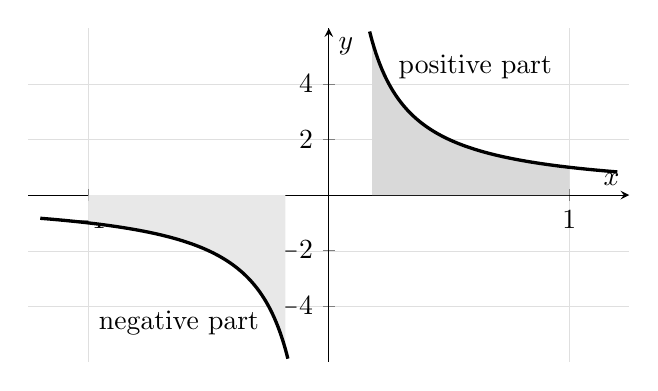
\begin{tikzpicture}
\begin{axis}[
    width=0.76\textwidth,
    height=0.48\textwidth,
    xmin=-1.25, xmax=1.25,
    ymin=-6, ymax=6,
    axis lines=middle,
    xlabel={\(x\)},
    ylabel={\(y\)},
    xtick={-1,0,1},
    ytick={-4,-2,0,2,4},
    grid=both,
    grid style={line width=.1pt, draw=gray!25},
    clip=true
]
\addplot[domain=-1:-0.18, samples=100, fill=gray!18, draw=none] {1/x} \closedcycle;
\addplot[domain=0.18:1, samples=100, fill=gray!30, draw=none] {1/x} \closedcycle;
\addplot[very thick, domain=-1.2:-0.17, samples=200] {1/x};
\addplot[very thick, domain=0.17:1.2, samples=200] {1/x};
\draw[dashed] (axis cs:0,-6) -- (axis cs:0,6);
\node[anchor=east] at (axis cs:-0.25,-4.6) {negative part};
\node[anchor=west] at (axis cs:0.25,4.6) {positive part};
\end{axis}
\end{tikzpicture}
\caption{The positive and negative pieces of \(1/x\) cancel symmetrically, but each piece has infinite size.}
\label{fig:principal-value-one-over-x}
\end{figure}

\begin{quote}
\textbf{Moral.}
For an improper integral over a singular point, each side must converge separately.
Cancellation of two infinite pieces is not convergence.
\end{quote}

\subsection{A CAS gives an antiderivative with the wrong domain}
\label{subsec:cas-wrong-domain-improper}

A computer algebra system may return an antiderivative that is correct only on part of
the real line, or correct only after choosing a complex logarithm branch.

Consider

\[
\int \frac{x}{x^2-1}\,dx.
\]

A symbolic system might return

\[
\frac12\ln(x^2-1)+C.
\]

Differentiating formally gives

\[
\frac12\cdot\frac{2x}{x^2-1}
=
\frac{x}{x^2-1}.
\]

But as a real-valued function,

\[
\ln(x^2-1)
\]

is defined only when

\[
x^2-1>0,
\]

that is, on

\[
(-\infty,-1)
\qquad\text{and}\qquad
(1,\infty).
\]

On the interval

\[
(-1,1),
\]

we have

\[
x^2-1<0.
\]

The real antiderivative there can be written as

\[
\frac12\ln(1-x^2)+C,
\]

because

\[
\frac{d}{dx}\left(\frac12\ln(1-x^2)\right)
=
\frac12\cdot\frac{-2x}{1-x^2}
=
\frac{x}{x^2-1}.
\]

The safest real formula on intervals where the integrand is defined is

\[
\boxed{
\int \frac{x}{x^2-1}\,dx
=
\frac12\ln|x^2-1|+C.
}
\]

Now evaluate

\[
\int_{-1/2}^{1/2}\frac{x}{x^2-1}\,dx.
\]

The integrand is continuous on \([-1/2,1/2]\), so the ordinary Fundamental Theorem
applies.  Using the real antiderivative,

\[
\int_{-1/2}^{1/2}\frac{x}{x^2-1}\,dx
=
\frac12\ln|x^2-1|\Big|_{-1/2}^{1/2}.
\]

At both endpoints,

\[
x^2-1=\frac14-1=-\frac34,
\]

so

\[
|x^2-1|=\frac34.
\]

Therefore

\[
\int_{-1/2}^{1/2}\frac{x}{x^2-1}\,dx
=
\frac12\ln\left(\frac34\right)
-
\frac12\ln\left(\frac34\right)
=
\boxed{0}.
\]

This also matches symmetry: the integrand is odd and the interval is symmetric.

\begin{quote}
\textbf{Moral.}
A symbolic antiderivative must be checked on the interval where it is used.  For real
calculus, logarithms often need absolute values or a different expression on a different
interval.
\end{quote}

\subsection{A trigonometric substitution triangle used outside its range}
\label{subsec:trig-substitution-wrong-range}

Trigonometric substitution is built from a triangle.  A triangle carries sign information.
If we reuse the same triangle on the wrong interval, the answer can change.

Earlier, for \(x>2\), we found

\[
\int \frac{\sqrt{x^2-4}}{x}\,dx
=
\sqrt{x^2-4}
-
2\arccos\left(\frac{2}{x}\right)
+C.
\]

That formula came from the substitution

\[
x=2\sec\theta,
\qquad
0\le\theta<\frac{\pi}{2}.
\]

On this range,

\[
\sec\theta\ge1,
\]

so

\[
x\ge2.
\]

The formula was derived on the interval \((2,\infty)\).

Now suppose \(x<-2\).  If we blindly use the same formula, it fails.

Let

\[
F_+(x)=\sqrt{x^2-4}-2\arccos\left(\frac2x\right).
\]

For \(x<-2\),

\[
\sqrt{1-\frac4{x^2}}
=
\frac{\sqrt{x^2-4}}{|x|}
=
-\frac{\sqrt{x^2-4}}{x},
\]

because \(x<0\).  Therefore

\[
\frac{d}{dx}\arccos\left(\frac2x\right)
=
-\frac{1}{\sqrt{1-\frac4{x^2}}}\left(-\frac2{x^2}\right)
=
-\frac{2}{x\sqrt{x^2-4}}.
\]

So

\[
F_+'(x)
=
\frac{x}{\sqrt{x^2-4}}
+
\frac{4}{x\sqrt{x^2-4}}.
\]

Thus

\[
F_+'(x)
=
\frac{x^2+4}{x\sqrt{x^2-4}},
\]

which is not

\[
\frac{\sqrt{x^2-4}}{x}
=
\frac{x^2-4}{x\sqrt{x^2-4}}.
\]

The formula from the \(x>2\) interval is not valid on \(x<-2\).

On \(x<-2\), one correct antiderivative is

\[
\boxed{
\sqrt{x^2-4}
+
2\arccos\left(\frac2x\right)
+C.
}
\]

Indeed, using the same derivative calculation,

\[
\frac{d}{dx}
\left[
\sqrt{x^2-4}
+
2\arccos\left(\frac2x\right)
\right]
=
\frac{x}{\sqrt{x^2-4}}
-
\frac{4}{x\sqrt{x^2-4}}
=
\frac{x^2-4}{x\sqrt{x^2-4}}.
\]

Therefore

\[
\frac{d}{dx}
\left[
\sqrt{x^2-4}
+
2\arccos\left(\frac2x\right)
\right]
=
\frac{\sqrt{x^2-4}}{x}.
\]

\begin{figure}[h]
\centering
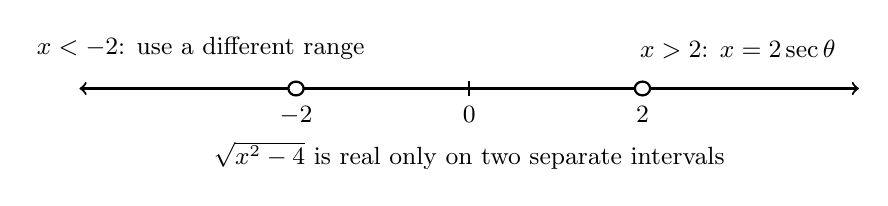
\begin{tikzpicture}[xscale=1.1, every node/.style={font=\small}]
  \draw[<->, thick] (-4.5,0) -- (4.5,0);
  \foreach \x/\lab in {-2/{-2},0/{0},2/{2}} {
    \draw[thick] (\x,0.09) -- (\x,-0.09);
    \node[below] at (\x,-0.1) {\(\lab\)};
  }

  \draw[very thick] (-4.2,0) -- (-2,0);
  \draw[very thick] (2,0) -- (4.2,0);
  \draw[fill=white, thick] (-2,0) circle (2.5pt);
  \draw[fill=white, thick] (2,0) circle (2.5pt);

  \node[above] at (3.1,0.25) {\(x>2\): \(x=2\sec\theta\)};
  \node[above] at (-3.1,0.25) {\(x<-2\): use a different range};
  \node[below] at (0,-0.55) {\(\sqrt{x^2-4}\) is real only on two separate intervals};
\end{tikzpicture}
\caption{The expression \(\sqrt{x^2-4}\) has two real branches of the domain.  A trigonometric substitution must respect the branch.}
\label{fig:trig-substitution-domain-branches}
\end{figure}

\begin{quote}
\textbf{Moral.}
An indefinite integral formula is usually valid on an interval.  When the domain has
separate pieces, such as

\[
(-\infty,-2)
\qquad\text{and}\qquad
(2,\infty),
\]

the same-looking formula may need different signs or different inverse functions on
different pieces.
\end{quote}

Improper integrals have given us one last lesson for exact integration: before computing,
ask where the integral is defined and what limit is being taken.

This chapter has focused on exact methods and convergence.  But exact antiderivatives
are not always available, and convergence alone may not give the number we need.  The
next question is practical:

\[
\boxed{
\text{How can we approximate an accumulated amount, and how can we control the error?}
}
\]

That question leads to numerical integration.

\section{Chapter review and discovery problems}
\label{sec:chapter-11-review-discovery}

This chapter began with a practical problem:

\[
\text{Applications give us integrals.  How do we evaluate them?}
\]

The answer was not one method.  It was a collection of ways to recognize structure.

Substitution reverses the chain rule.  Integration by parts reverses the product rule.
Trigonometric identities reshape trigonometric expressions.  Trigonometric substitution
uses right triangles to simplify square roots.  Partial fractions split rational functions into
simpler pieces.  Improper integrals add one more demand: before evaluating, we must ask
whether the accumulated amount is finite.

So the main lesson is not a list of tricks.  It is a habit:

\[
\boxed{
\text{Read the integrand before choosing a method.}
}
\]

\subsection{The chapter in one map}
\label{subsec:chapter-11-one-map}

A good integration method answers a specific question about the integrand.

\begin{center}
\begin{tabular}{p{0.28\textwidth}|p{0.34\textwidth}|p{0.30\textwidth}}
\textbf{What you see} & \textbf{Question to ask} & \textbf{Likely method} \\ \hline
An inside function and its derivative & Is the chain rule hiding here? & Substitution \\[5pt]
A product where one factor simplifies when differentiated & Did the product rule create this? & Integration by parts \\[5pt]
Powers of \(\sin x\), \(\cos x\), \(\tan x\), or \(\sec x\) & Can I save a differential and rewrite the rest? & Trigonometric identities \\[5pt]
\(\sqrt{a^2-x^2}\), \(\sqrt{a^2+x^2}\), or \(\sqrt{x^2-a^2}\) & Which Pythagorean identity matches the square root? & Trigonometric substitution \\[5pt]
A quotient of polynomials & Is the rational function proper, and how does the denominator factor? & Partial fractions \\[5pt]
An infinite interval or an infinite discontinuity & Does the limiting accumulated amount exist? & Improper integral tests \\[5pt]
A strange but important integral & Does an elementary antiderivative exist? & Special functions or numerical methods
\end{tabular}
\end{center}

The same integral may yield to more than one method.  The goal is not to find the only
path.  The goal is to find a path that makes the structure visible.

\begin{figure}[h]
\centering
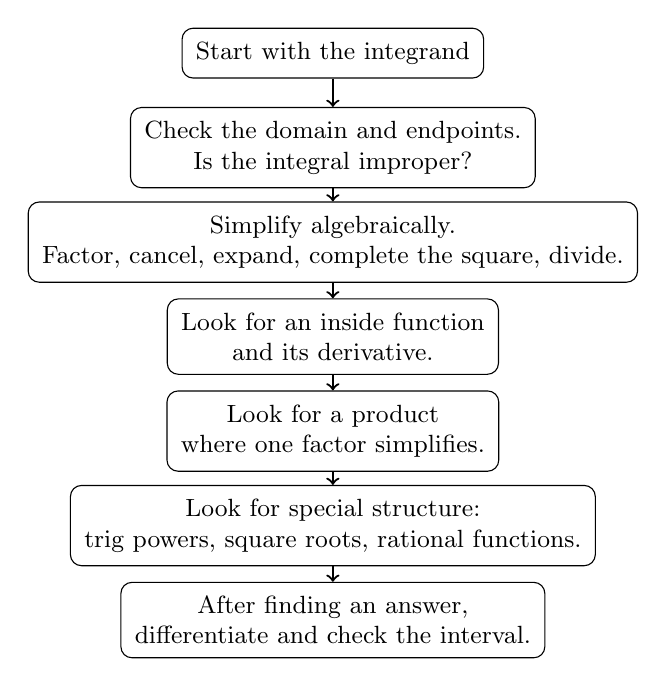
\begin{tikzpicture}[
  node distance=1.2cm,
  box/.style={draw, rounded corners, align=center, inner sep=5pt, font=\small},
  arrow/.style={->, thick}
]
\node[box] (start) {Start with the integrand};
\node[box, below of=start] (domain) {Check the domain and endpoints.\\Is the integral improper?};
\node[box, below of=domain] (algebra) {Simplify algebraically.\\Factor, cancel, expand, complete the square, divide.};
\node[box, below of=algebra] (sub) {Look for an inside function\\and its derivative.};
\node[box, below of=sub] (parts) {Look for a product\\where one factor simplifies.};
\node[box, below of=parts] (special) {Look for special structure:\\trig powers, square roots, rational functions.};
\node[box, below of=special] (check) {After finding an answer,\\differentiate and check the interval.};

\draw[arrow] (start) -- (domain);
\draw[arrow] (domain) -- (algebra);
\draw[arrow] (algebra) -- (sub);
\draw[arrow] (sub) -- (parts);
\draw[arrow] (parts) -- (special);
\draw[arrow] (special) -- (check);
\end{tikzpicture}
\caption{A practical order of questions for integration.  The order is flexible, but the first step is always to read the integrand.}
\label{fig:chapter-11-integration-map}
\end{figure}

\subsection{Essential formulas and patterns}
\label{subsec:chapter-11-essential-formulas}

\paragraph{Integration by parts.}

\[
\boxed{
\int u\,dv=uv-\int v\,du.
}
\]

For definite integrals,

\[
\boxed{
\int_a^b u\,dv=\bigl[uv\bigr]_a^b-\int_a^b v\,du.
}
\]

The product term

\[
\bigl[uv\bigr]_a^b
\]

is a boundary term.

\paragraph{Trigonometric identities.}

\[
\sin^2x+\cos^2x=1,
\]

\[
1+\tan^2x=\sec^2x,
\]

\[
\sin^2x=\frac{1-\cos2x}{2},
\qquad
\cos^2x=\frac{1+\cos2x}{2}.
\]

Product-to-sum identities include

\[
\sin A\cos B=\frac12\bigl(\sin(A+B)+\sin(A-B)\bigr),
\]

\[
\cos A\cos B=\frac12\bigl(\cos(A-B)+\cos(A+B)\bigr),
\]

and

\[
\sin A\sin B=\frac12\bigl(\cos(A-B)-\cos(A+B)\bigr).
\]

\paragraph{Trigonometric substitution patterns.}

\[
\sqrt{a^2-x^2}
\quad\Longrightarrow\quad
x=a\sin\theta,
\]

\[
\sqrt{a^2+x^2}
\quad\Longrightarrow\quad
x=a\tan\theta,
\]

\[
\sqrt{x^2-a^2}
\quad\Longrightarrow\quad
x=a\sec\theta.
\]

The substitution is not complete until \(dx\) changes too.

\[
x=a\sin\theta
\quad\Longrightarrow\quad
dx=a\cos\theta\,d\theta,
\]

\[
x=a\tan\theta
\quad\Longrightarrow\quad
dx=a\sec^2\theta\,d\theta,
\]

\[
x=a\sec\theta
\quad\Longrightarrow\quad
dx=a\sec\theta\tan\theta\,d\theta.
\]

\paragraph{Partial fractions.}

A proper rational function with distinct linear factors has the form

\[
\frac{P(x)}{(x-r_1)(x-r_2)\cdots(x-r_n)}
=
\frac{A_1}{x-r_1}
+
\frac{A_2}{x-r_2}
+\cdots+
\frac{A_n}{x-r_n}.
\]

A repeated linear factor contributes every power:

\[
(x-r)^m
\quad\Longrightarrow\quad
\frac{A_1}{x-r}
+
\frac{A_2}{(x-r)^2}
+\cdots+
\frac{A_m}{(x-r)^m}.
\]

An irreducible quadratic factor contributes a linear numerator:

\[
ax^2+bx+c
\quad\Longrightarrow\quad
\frac{Ax+B}{ax^2+bx+c}.
\]

\paragraph{Improper integrals.}

An integral over an infinite interval is a limit:

\[
\boxed{
\int_a^\infty f(x)\,dx
=
\lim_{t\to\infty}\int_a^t f(x)\,dx.
}
\]

An integral with an infinite discontinuity at an endpoint is also a limit:

\[
\boxed{
\int_a^b f(x)\,dx
=
\lim_{t\to a^+}\int_t^b f(x)\,dx
}
\]

when the singularity is at \(a\).

The \(p\)-integrals are the main comparison family:

\[
\boxed{
\int_1^\infty \frac{dx}{x^p}
\text{ converges exactly when }p>1,
}
\]

and

\[
\boxed{
\int_0^1 \frac{dx}{x^p}
\text{ converges exactly when }p<1.
}
\]

\subsection{Concept check}
\label{subsec:chapter-11-concept-check}

Answer these in words before doing calculations.

\begin{enumerate}
\item Why does integration by parts reverse the product rule?

\item In

\[
\int u\,dv=uv-\int v\,du,
\]

what makes one choice of \(u\) and \(dv\) better than another?

\item Why can

\[
\int \ln x\,dx
\]

be treated as an integration by parts problem?

\item In a trigonometric integral involving powers of sine and cosine, why is an odd
power useful?

\item Why do half-angle identities appear when both powers of sine and cosine are even?

\item What right-triangle identity is behind the substitution

\[
x=a\sin\theta
\]

for expressions involving

\[
\sqrt{a^2-x^2}?
\]

\item Why must a rational function be proper before partial fractions begin?

\item Why does an irreducible quadratic factor need a linear numerator in partial
fractions?

\item Why is

\[
\int_{-1}^{1}\frac1x\,dx
\]

not equal to \(0\), even though the graph has symmetric positive and negative parts?

\item What is the difference between saying

\[
\int e^{-x^2}\,dx
\]

has no elementary antiderivative and saying the integral does not exist?
\end{enumerate}

\subsection{Skills: choose the method}
\label{subsec:skills-choose-method}

For each integral, identify the method you would try first.  Do not evaluate the integral
yet.  Explain the clue that led to your choice.

\begin{enumerate}
\item
\[
\int x e^{x^2}\,dx
\]

\item
\[
\int x e^x\,dx
\]

\item
\[
\int x^2\ln x\,dx
\]

\item
\[
\int \sin^5x\cos^2x\,dx
\]

\item
\[
\int \sin^2x\cos^2x\,dx
\]

\item
\[
\int \tan^3x\sec^4x\,dx
\]

\item
\[
\int \sqrt{16-x^2}\,dx
\]

\item
\[
\int \frac{dx}{\sqrt{x^2+9}}
\]

\item
\[
\int \frac{x+1}{x^2-5x+6}\,dx
\]

\item
\[
\int \frac{x^3}{x^2+1}\,dx
\]

\item
\[
\int \sin(4x)\cos(7x)\,dx
\]

\item
\[
\int_1^\infty \frac{dx}{x^{3/2}}
\]
\end{enumerate}

\subsection{Mixed practice}
\label{subsec:chapter-11-mixed-practice}

Evaluate the following indefinite integrals.  Check each answer by differentiating.

\begin{enumerate}
\item
\[
\int x\sin x\,dx
\]

\item
\[
\int x^2e^x\,dx
\]

\item
\[
\int x\arctan x\,dx
\]

\item
\[
\int \ln(3x)\,dx
\]

\item
\[
\int e^{2x}\cos(3x)\,dx
\]

\item
\[
\int \sin^3x\cos^4x\,dx
\]

\item
\[
\int \cos^5x\,dx
\]

\item
\[
\int \sin^2(3x)\,dx
\]

\item
\[
\int \tan^4x\sec^2x\,dx
\]

\item
\[
\int \sec^2x\tan^3x\,dx
\]

\item
\[
\int \sqrt{9-x^2}\,dx
\]

\item
\[
\int \frac{dx}{\sqrt{25-x^2}}
\]

\item
\[
\int \frac{dx}{x^2+4x+13}
\]

\item
\[
\int \frac{3x+1}{(x-2)(x+1)}\,dx
\]

\item
\[
\int \frac{x^2+1}{x^3-x}\,dx
\]

\item
\[
\int \frac{x^3}{x^2+1}\,dx
\]

\item
\[
\int \frac{dx}{1+e^x}
\]

\item
\[
\int \sin(4x)\cos(7x)\,dx
\]

\item
\[
\int \frac{x}{x^2-4x+5}\,dx
\]

\item
\[
\int \frac{dx}{x^2\sqrt{x^2-1}},
\qquad x>1.
\]
\end{enumerate}

\subsection{Definite integrals}
\label{subsec:chapter-11-definite-integrals}

Evaluate the following definite integrals.  Use endpoint terms carefully when using
integration by parts.

\begin{enumerate}
\item
\[
\int_0^1 xe^x\,dx
\]

\item
\[
\int_0^\pi x\sin x\,dx
\]

\item
\[
\int_0^{\pi/2}\sin^3x\cos^2x\,dx
\]

\item
\[
\int_0^{\pi/4}\tan^3x\,dx
\]

\item
\[
\int_0^2 \frac{x+1}{x^2+2x+2}\,dx
\]

\item
\[
\int_0^1 \frac{dx}{x^2+4}
\]

\item
\[
\int_0^1 \sqrt{1-x^2}\,dx
\]

\item
\[
\int_1^2 \frac{x^2+1}{x^3+x}\,dx
\]
\end{enumerate}

\subsection{Improper integral practice}
\label{subsec:chapter-11-improper-practice}

For each integral, decide whether it converges or diverges.  If it converges and the value
can be found with the methods of this chapter, evaluate it.

\begin{enumerate}
\item
\[
\int_1^\infty \frac{dx}{x^{3/2}}
\]

\item
\[
\int_1^\infty \frac{dx}{\sqrt{x}}
\]

\item
\[
\int_0^1 \frac{dx}{x^{2/3}}
\]

\item
\[
\int_0^1 \frac{dx}{x}
\]

\item
\[
\int_{-\infty}^{\infty}\frac{dx}{1+x^2}
\]

\item
\[
\int_{-\infty}^{\infty}\frac{x}{1+x^2}\,dx
\]

\item
\[
\int_2^\infty \frac{5x+1}{x^3+4}\,dx
\]

\item
\[
\int_2^\infty \frac{x^2+1}{x^3+1}\,dx
\]

\item
\[
\int_0^\infty e^{-3x}\,dx
\]

\item
\[
\int_0^\infty xe^{-x}\,dx
\]

\item
\[
\int_0^1 \frac{\ln x}{\sqrt{x}}\,dx
\]

\item
\[
\int_1^\infty \frac{1+\sin^2x}{x}\,dx
\]
\end{enumerate}

\subsection{Warning review}
\label{subsec:chapter-11-warning-review}

Each item below contains a common error.  Find it and correct it.

\begin{enumerate}
\item A student writes

\[
\int x e^x\,dx
=
\frac{x^2}{2}e^x+C.
\]

Explain why this cannot be correct.

\item A student evaluates

\[
\int_{-1}^{1}\frac{dx}{x^2}
\]

by writing

\[
\left[-\frac1x\right]_{-1}^1=-2.
\]

Where did the calculation fail?

\item A student writes

\[
\int_0^1 \frac{dx}{\sqrt{x}}
=
\left[2\sqrt{x}\right]_0^1
=
2,
\]

without mentioning a limit.  The answer is correct.  What is missing from the reasoning?

\item A student writes

\[
\int \frac{x}{x^2-1}\,dx
=
\frac12\ln(x^2-1)+C
\]

and then uses it on the interval \((-1,1)\).  What is wrong, and how should the formula
be written?

\item A student tries

\[
x=3\sin\theta
\]

for

\[
\sqrt{x^2+9}.
\]

Why is this not the matching trigonometric substitution?

\item A computer algebra system returns a complicated expression for an antiderivative.
What two checks should be done before trusting it?

\item A graph suggests that

\[
\int_{-10}^{10} \frac{\sin x}{x}\,dx
\]

has a finite value.  Why does this evidence not automatically answer whether

\[
\int_{-\infty}^{\infty} \frac{\sin x}{x}\,dx
\]

converges as an improper integral?
\end{enumerate}

\subsection{Project: build an integration decision tree}
\label{subsec:project-build-integration-decision-tree}

Create a one-page decision tree for choosing an integration method.

Your decision tree should include at least the following methods:

\[
\text{substitution, parts, trigonometric identities, trigonometric substitution,}
\]

\[
\text{partial fractions, improper integral tests, and numerical approximation.}
\]

Use the following integrals as test cases.

\[
\int x\cos(x^2)\,dx,
\qquad
\int x\cos x\,dx,
\qquad
\int \ln x\,dx,
\]

\[
\int \sin^4x\cos^3x\,dx,
\qquad
\int \sin^2x\,dx,
\qquad
\int \frac{dx}{\sqrt{4-x^2}},
\]

\[
\int \sqrt{x^2+1}\,dx,
\qquad
\int \frac{x+4}{x^2-x-2}\,dx,
\qquad
\int \frac{x^2}{x^2+1}\,dx,
\]

\[
\int_1^\infty \frac{dx}{x^p},
\qquad
\int e^{-x^2}\,dx,
\qquad
\int_0^1 e^{-x^2}\,dx.
\]

Your report should answer these questions.

\begin{enumerate}
\item Which questions does your decision tree ask first?

\item Which examples go down more than one possible branch?

\item Give one example where substitution is shorter than trigonometric substitution.

\item Give one example where algebra before calculus makes the integral much easier.

\item Give one example where exact elementary integration is not available, but the
definite integral still has meaning.

\item Revise your decision tree after testing it.  What changed?
\end{enumerate}

\begin{quote}
\textbf{What the project tests.}
A decision tree is useful only if it survives examples.  The goal is not to force every
integral into one rigid path, but to learn which questions reveal structure.
\end{quote}

\subsection{Project: compare human and CAS antiderivatives}
\label{subsec:project-compare-human-cas}

Use a computer algebra system to evaluate several integrals from this chapter.  For each
one, compare the computer's answer with a human answer.

Use at least six integrals, including one from each group.

\begin{center}
\begin{tabular}{c|p{0.65\textwidth}}
\textbf{Group} & \textbf{Choose at least one} \\ \hline
Integration by parts & \(\displaystyle \int x e^x\,dx\), \(\displaystyle \int x\ln x\,dx\), \(\displaystyle \int x\arctan x\,dx\) \\[6pt]
Trigonometric identities & \(\displaystyle \int \sin^4x\,dx\), \(\displaystyle \int \sin(3x)\cos(5x)\,dx\) \\[6pt]
Trigonometric substitution & \(\displaystyle \int \sqrt{9-x^2}\,dx\), \(\displaystyle \int \frac{dx}{\sqrt{x^2+4}}\) \\[6pt]
Partial fractions & \(\displaystyle \int \frac{dx}{x^2-1}\), \(\displaystyle \int \frac{x+1}{x^2+x-2}\,dx\) \\[6pt]
Improper or special-function issue & \(\displaystyle \int_0^\infty e^{-x}\,dx\), \(\displaystyle \int e^{-x^2}\,dx\)
\end{tabular}
\end{center}

For each integral, include the following.

\begin{enumerate}
\item The answer produced by the computer algebra system.

\item A human solution or a human explanation of the method.

\item A derivative check of the returned antiderivative.

\item A note about the interval where the answer is valid.

\item A note about whether logarithms need absolute values.

\item If the computer uses a special function, explain what accumulation that special
function represents.
\end{enumerate}

\begin{quote}
\textbf{What the project tests.}
A computer can manipulate symbols quickly.  It cannot replace the mathematical
questions:

\[
\text{Does the answer differentiate correctly?}
\]

\[
\text{On what interval is it valid?}
\]

\[
\text{Does it explain the accumulated quantity?}
\]
\end{quote}

\subsection{Challenge problems}
\label{subsec:chapter-11-challenge-problems}

These problems combine several ideas from the chapter.

\begin{enumerate}
\item Evaluate

\[
\int x^3e^{x^2}\,dx.
\]

Use substitution first, then algebra.

\item Evaluate

\[
\int \frac{x^2}{x^2+2x+2}\,dx.
\]

Hint: rewrite the numerator in terms of the denominator and its derivative.

\item Evaluate

\[
\int \frac{dx}{x^4-1}.
\]

Begin by factoring the denominator over the real numbers.

\item Evaluate

\[
\int_0^1 x\ln(1+x)\,dx.
\]

Use integration by parts.

\item Determine all real numbers \(p\) for which

\[
\int_0^1 \frac{\ln x}{x^p}\,dx
\]

converges.

\item Show that

\[
\int_1^\infty \frac{dx}{x^p+x}
\]

converges exactly when \(p>1\).

\item Evaluate

\[
\int \frac{dx}{\sqrt{x^2-4}},
\qquad x>2.
\]

Then check your answer by differentiating.

\item For \(a>0\), evaluate

\[
\int_0^a \sqrt{a^2-x^2}\,dx
\]

using geometry and then using trigonometric substitution.  Explain why the two answers
must agree.

\item Let

\[
F(x)=\int_0^x e^{-t^2}\,dt.
\]

Show that \(F\) is increasing on all of \(\mathbb R\), and that \(F\) is concave down for
\(x>0\) and concave up for \(x<0\).  You do not need an elementary formula for \(F\).

\item Suppose \(f\) is positive, decreasing, and continuous on \([1,\infty)\).  Explain why
the convergence of

\[
\int_1^\infty f(x)\,dx
\]

depends only on the tail behavior of \(f\), not on any finite beginning interval
\([1,N]\).
\end{enumerate}

\subsection{Where this points}
\label{subsec:chapter-11-hook-numerical-integration}

Exact integration is powerful, but it is not the whole story.

Some integrals have elementary antiderivatives:

\[
\int x e^x\,dx,
\qquad
\int \frac{x+1}{x^2-1}\,dx.
\]

Some have antiderivatives that require special functions:

\[
\int e^{-x^2}\,dx.
\]

Some come from data instead of formulas.  A speedometer may give readings every
second.  A thermometer may give temperatures every hour.  A sensor may give force
measurements at discrete positions.  In those cases, there may be no formula to
antidifferentiate.

But the accumulated amount may still be exactly what we need.

\[
\int_0^1 e^{-x^2}\,dx
\]

is a real number.  The length

\[
\int_0^\pi \sqrt{1+\cos^2x}\,dx
\]

is a real length.  The work computed from measured force data is real work.

So the next question is not

\[
\text{Can we always find an exact antiderivative?}
\]

The answer is no.

The better question is

\[
\boxed{
\text{How can we approximate an integral, and how can we know how accurate the approximation is?}
}
\]

That question leads to numerical integration, error estimates, and computation.